\documentclass[9pt,twocolumn,twoside]{pnas-new}
% Use the lineno option to display guide line numbers if required.
% Note that the use of elements such as single-column equations
% may affect the guide line number alignment.

\templatetype{pnasresearcharticle} % Choose template
% {pnasresearcharticle} = Template for a two-column research article
% {pnasmathematics} = Template for a one-column mathematics article
% {pnasinvited} = Template for a PNAS invited submission

\usepackage{pslatex}
\usepackage{amsfonts}
\usepackage{graphicx}
\usepackage{color}
\usepackage{todonotes}
\usepackage{dsfont}
\usepackage{array}
\usepackage{textcomp}
\usepackage{multirow}
\usepackage{subfig}
\usepackage{todonotes}
\usepackage{hyperref}
\usepackage{booktabs}
\usepackage{xcolor}
\tolerance=1
\emergencystretch=\maxdimen
\hyphenpenalty=10000
\hbadness=10000

\newcommand{\mwu}[1]{{\color{red}{[mwu: #1]}}}
\newcommand{\rdh}[1]{{\color{blue}{[rdh: #1]}}}
\definecolor{Green}{RGB}{50,200,50}
\newcommand{\ndg}[1]{\textcolor{Green}{[ndg: #1]}}  

\title{Pragmatic inference and visual abstraction enable contextual flexibility during visual communication}

% Use letters for affiliations, numbers to show equal authorship (if applicable) and to indicate the corresponding author

\author[a,c,1]{Judith E. Fan}
\author[a]{Robert X.D. Hawkins}
\author[b]{Mike Wu}
\author[a,b]{Noah D. Goodman}

\affil[a]{Department of Psychology, Stanford University}
\affil[b]{Department of Computer Science, Stanford University}
\affil[c]{Department of Psychology, University of California, San Diego}

% Please give the surname of the lead author for the running footer
\leadauthor{Fan}

\significancestatement{Drawing is a versatile tool for communication, spanning detailed renderings and simple sketches. Even the same object can be drawn in many ways, depending on the context. How do people decide how to draw in order to be understood? We collected a large number of drawings in different contexts and found that people adapted their drawings accordingly, producing detailed drawings when necessary, but simpler drawings when sufficient. To explain this contextual flexibility, we developed a computational model combining: the capacity to perceive the correspondence between an object and drawing with the ability to infer what information is relevant to the viewer in context. Our results suggest drawing may be so versatile because humans possess these two capacities.}

% Please include corresponding author, author contribution and author declaration information
\authorcontributions{J.E.F and R.X.D.H. designed and conducted human experiments, J.E.F, R.X.D.H, and M.W. analyzed data and performed computational modeling. J.E.F, R.X.D.H, M.W., and N.D.G. formulated models, interpreted results, and wrote the paper.}
\authordeclaration{The authors declare no conflict of interest.}
\correspondingauthor{\textsuperscript{1}To whom correspondence should be addressed. E-mail: jefan@stanford.edu}

% Keywords are not mandatory, but authors are strongly encouraged to provide them. If provided, please include two to five keywords, separated by the pipe symbol, e.g:
\keywords{drawing $|$ social cognition $|$ perception $|$ deep learning $|$ probabilistic models}

\begin{abstract}
Visual modes of communication are ubiquitous in modern life --- from maps to data plots to political cartoons. 
Here we investigate drawing, the most basic form of visual communication. 
Communicative drawing poses a core challenge for theories of how visual perception and social cognition interact, requiring a detailed understanding of how sensory information and social context jointly determine what information is relevant to communicate. 
Participants (N=192) were paired in an online environment to play a sketching-based reference game. On each trial, both participants were shown the same four objects, but in different locations. The sketcher's goal was to draw one of these objects --- the target --- so that the viewer could select it from the array. 
There were two types of trials: close, where objects belonged to the same basic-level category, and far, where objects belonged to different categories. 
We found that people exploited information in common ground with their partner to efficiently communicate about the target: on far trials, sketchers achieved high recognition accuracy while applying fewer strokes, using less ink, and spending less time on their drawings than on close trials. 
We hypothesized that humans succeed in this task by recruiting two core faculties: (1) visual abstraction, the capacity to perceive the correspondence between an object and a drawing of it; and (2) pragmatic inference, the ability to infer what information would help a viewer distinguish the target from distractors. 
To evaluate this hypothesis, we developed a computational model of the sketcher that embodied both faculties, instantiated as a deep convolutional neural network nested within a probabilistic program. 
We found that this model fit human data well and outperformed lesioned variants. 
Together, this work provides the first algorithmically explicit theory of how perception and social cognition jointly support contextual flexibility in visual communication.
\end{abstract}

\dates{This manuscript was compiled on \today}
\doi{\url{www.pnas.org/cgi/doi/10.1073/pnas.XXXXXXXXXX}}

\begin{document}

% Optional adjustment to line up main text (after abstract) of first page with line numbers, when using both lineno and twocolumn options.
% You should only change this length when you've finalised the article contents.
\verticaladjustment{-2pt}

\maketitle
\thispagestyle{firststyle}
\ifthenelse{\boolean{shortarticle}}{\ifthenelse{\boolean{singlecolumn}}{\abscontentformatted}{\abscontent}}{}

\noindent \dropcap{F}rom ancient etchings on cave walls to modern digital displays, the ability to externalize our thoughts in visual form lies at the heart of key human innovations (e.g., painting, cartography, data visualization), and forms the foundation for the cultural transmission of knowledge \cite{tomasello2009cultural,donald1991origins}. 
Perhaps the most basic and versatile visualization technique is drawing, the earliest examples of which date to at least 40,000 years ago \cite{hoffmann2018u,Aubert:2014jy}, and which can yield images ranging from photorealistic renderings to schematic diagrams. 
Even in the simple case of sketching an object in the world, there are countless ways of depicting that object. 
How do drawings, despite spanning such a broad range of appearances, reliably convey meaning? 

On the one hand, recent work in computational vision suggests that the identity of an object depicted in a drawing can be derived from its visual properties alone \cite{FanCommon2018}.
These results are consistent with evidence from other domains, including developmental, cross-cultural, and comparative studies of drawing perception. 
For example, human infants \cite{hochberg1962pictorial}, people living in remote regions without pictorial art traditions and without substantial contact with Western visual media \cite{kennedy1975outline}, and higher non-human primates \cite{tanaka2007recognition} are able to recognize line drawings of familiar objects, even without prior experience with drawings.
Together, these findings suggest that the ability to perceive the correspondence between drawings and real-world objects arises from a general-purpose neural architecture evolved to handle variation in natural visual inputs \cite{Sayim:2011bz,gibson2014ecological}. 

On the other hand, influential work in philosophy has emphasized the role of cultural and social context in determining how drawings denote objects \cite{goodman1976languages}.
This perspective is consistent with the observation of substantial variation in pictorial art traditions across cultures \cite{gombrich1989story,gombrich1969art}, and the emergence of culturally-specific conventions for encoding meaning in pictorial form \cite{boltz1994origin,allen2000middle}. 
Further support for the importance of social context for determining pictorial meaning has also come from recent laboratory studies of visual communication, which have found that pairs of interacting participants can learn to produce drawings that are referentially meaningful to their partner in context, even when these drawings do not strongly resemble any particular real-world referent out of context \cite{Garrod:2007wk,fay2010interactive,Galantucci:2005uh}. 

Towards reconciling these perspectives, the current paper is guided by the overarching hypothesis that visual information and social context jointly determine the relationship between a drawing and the object it depicts.  
To evaluate this hypothesis, we investigated how the drawings people produce during visual communication varied across different contexts, and found that people spontaneously modulated how much time and ink they invested in their drawings in order to be sufficiently informative in context.
To explain these findings, we developed a computational model of visual communication that embodied two core faculties: visual abstraction, the capacity to judge the correspondence between a real-world object and a drawing of it; and pragmatic inference, the ability to infer what information is not only \textit{valid} to include in a drawing, but also \textit{relevant} in context  \cite{goodman2016pragmatic,grice1975syntax,abell2009canny}.
This model was instantiated as a deep convolutional neural network visual encoder nested within a probabilistic program that inferred which drawings would be most informative in context.
We found that our full model fits the data well and outperformed lesioned variants, providing a first algorithmically explicit theory of how perception and social cognition jointly support contextual flexibility in visual communication.

\section*{Results}

\subsection*{Effect of context manipulation on communication task performance}

%%%%% List of results figures
%% Figure 1: Task Display & Design & example drawings
%% Figure 2: Sketch Gallery
%% Figure 3: Communication Game Task Performance & Recognition Task Performance
%% Figure 4: Model schematic
%% Figure 5: Model comparison & evaluation (absolute performance) -- human+RSA (2 production x 2 pragmatics = 4 bars) + VGG+RSA (2 production x 2 pragmatics x 3 perception = 12 bars)

%% Supplemental 1: Perceptual similarity -- maybe confusion matrix
%% Supplemental 2: Param posteriors
%% Supplemental 3: Error analysis for each lesioned versions

To investigate visual communication in a naturalistic yet controlled setting, we employ a sketching-based reference game paradigm.
This reference game involves two players: a \textit{sketcher} who aims to help a \textit{viewer} pick out a target object from an array of distractor objects by representing it in a sketch. 
This basic arrangement can be traced back to the language games explored by \citep{wittgenstein1953philosophical} and \citep{Lewis69_Convention}. 
Such games have proven to be a valuable tool for eliciting pragmatic inferences about \textit{language} use in context, and to make quantitative measurements of the behavioral consequences of these inferences \cite{goodman2016pragmatic,kao2014formalizing,goodman2013knowledge,frank2012predicting}. 
Here we generalize this methodology to understand how sketchers account for information in common ground with their viewer in order to produce sketches that are informative \cite{grice1975syntax,wilson1986relevance} yet parsimonious \cite{zipf1936psycho}.
\begin{figure}[htbp]
\centering
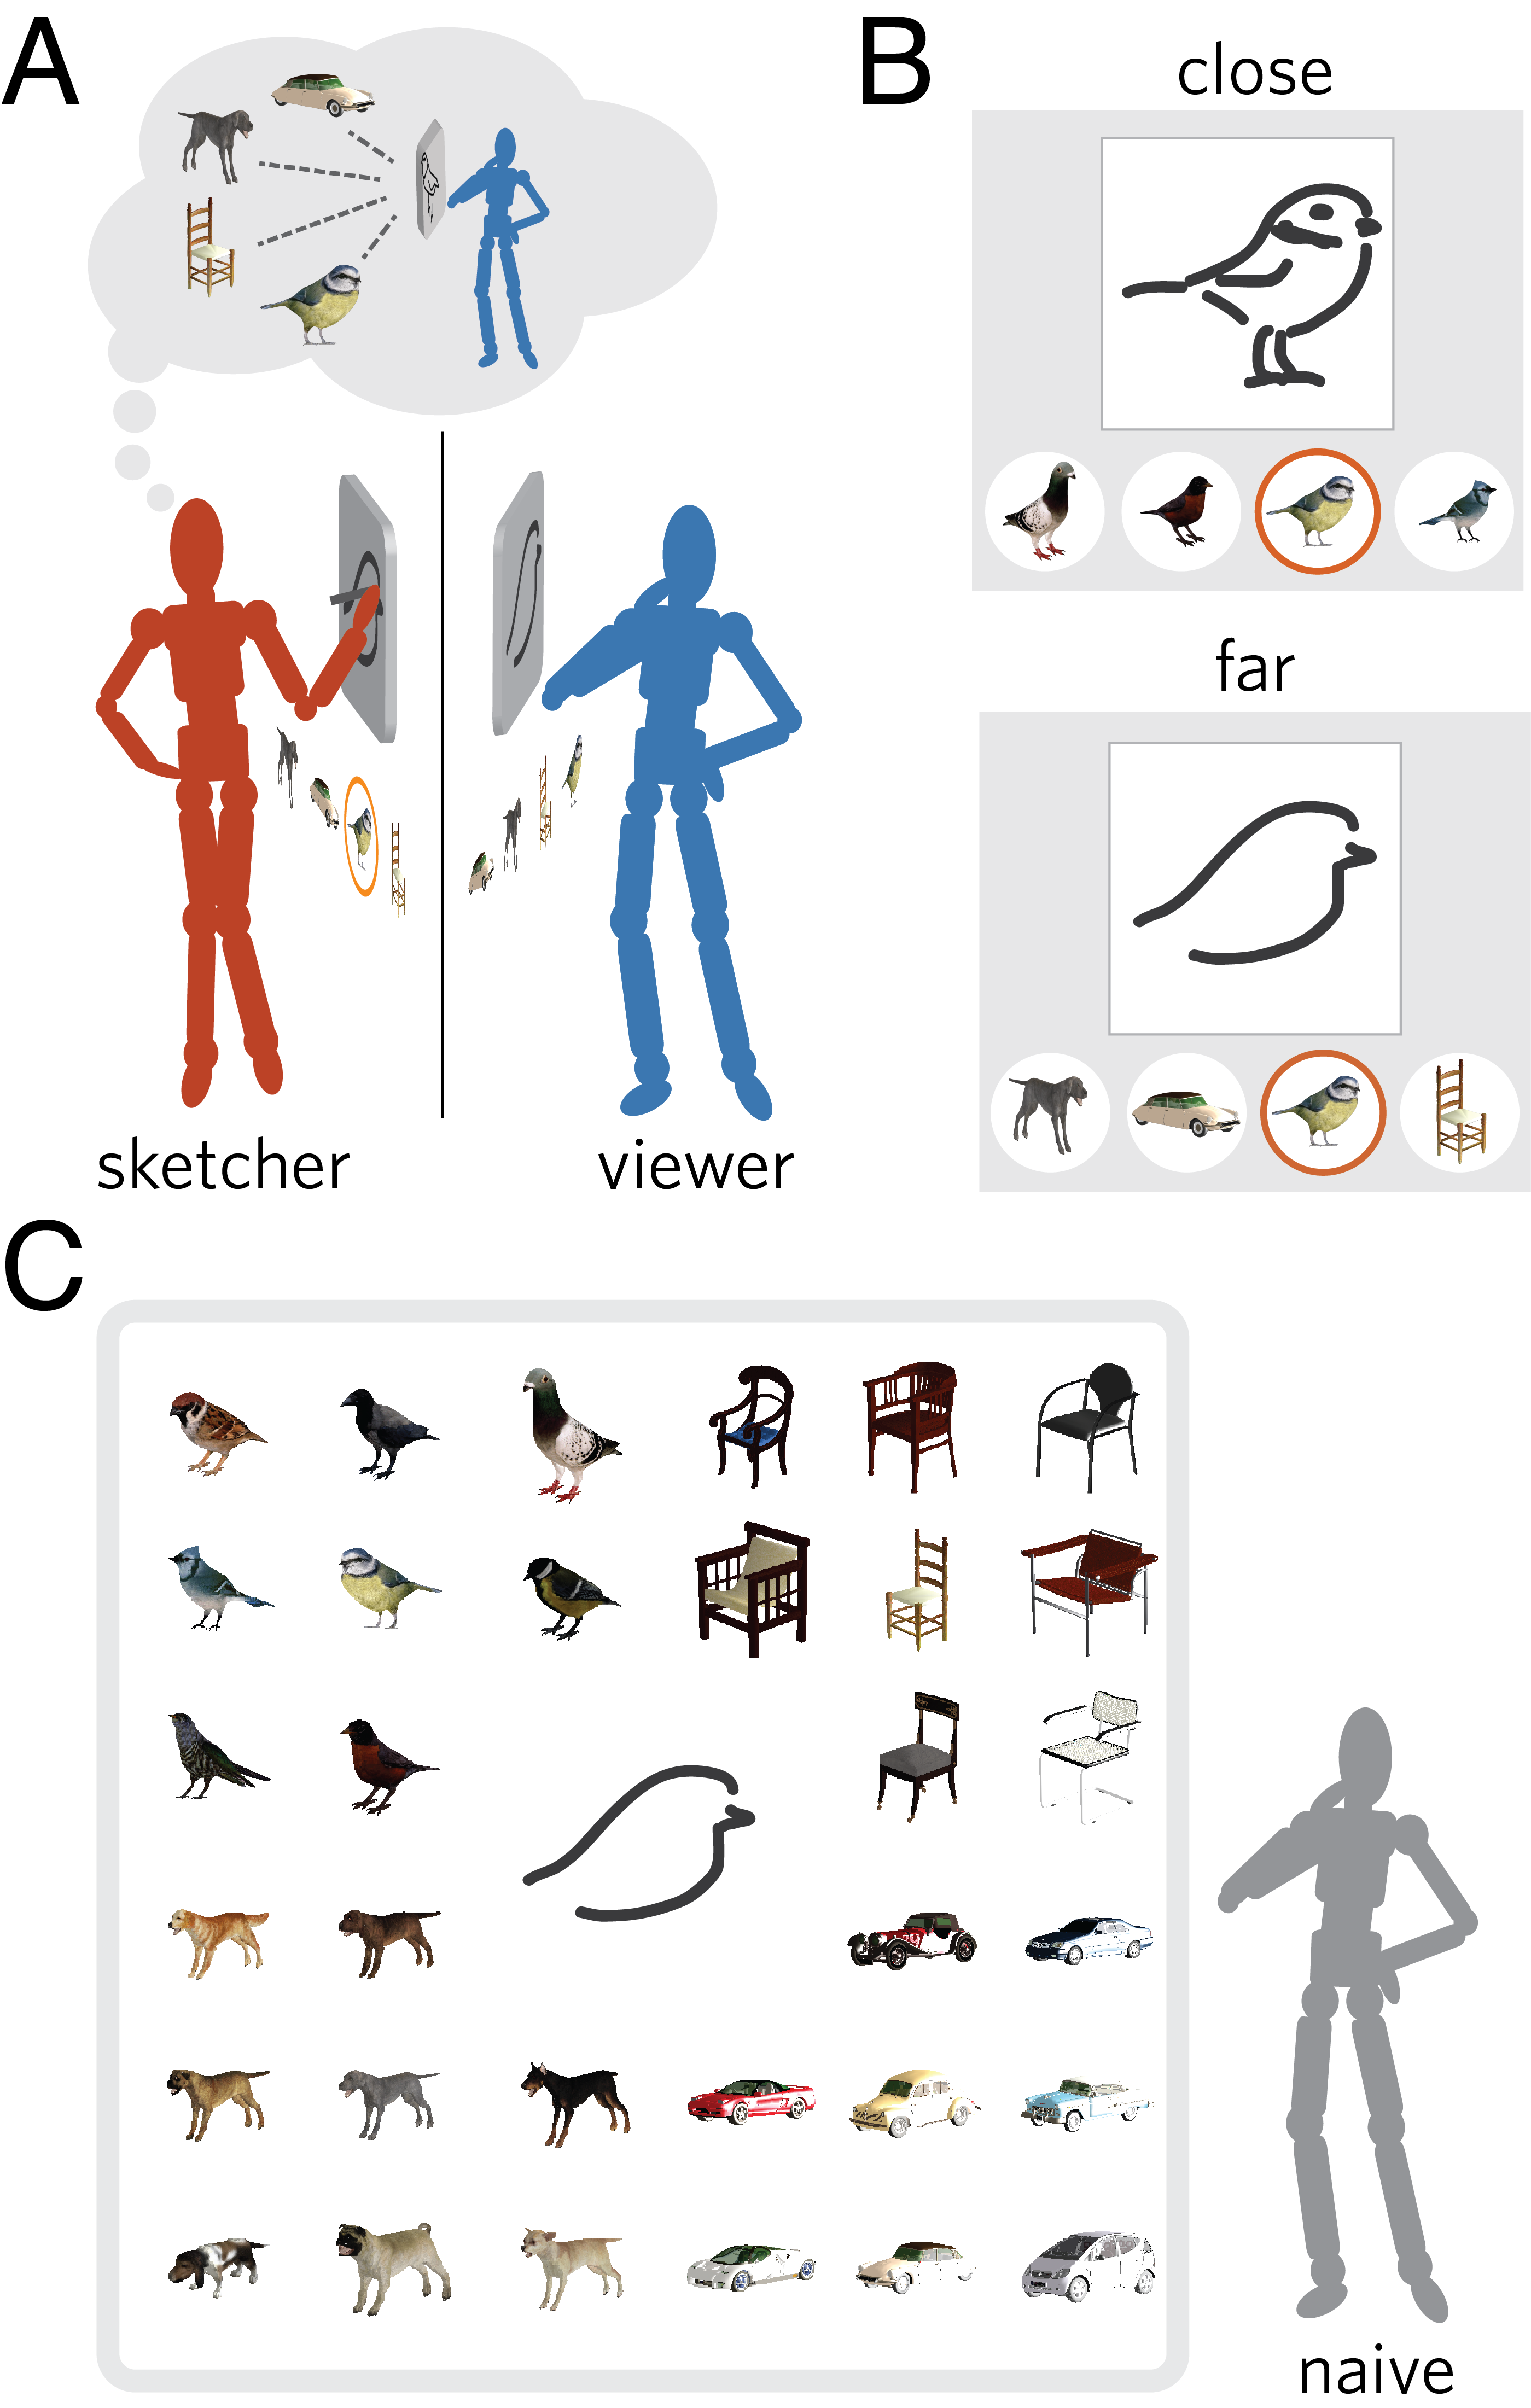
\includegraphics[width=0.35\textwidth]{figures/1_task_display_alt.png}
\caption{(A) Communication task. Participants were paired in an online environment to play a sketching-based reference game and assigned the roles of \textit{sketcher} and \textit{viewer}. On each trial, the sketcher's goal was to draw one of these objects so that the viewer could distinguish the target from three distractor objects. (B) Context manipulation. Distractor similarity to target was manipulated across two context conditions: in close contexts, the target and distractors belonged to the same basic-level category, while in far contexts, the target and distractors all belonged to different basic-level categories. (C) Recognition task. Naive participants were presented with a randomly sampled sketch from the communication experiment and an array containing all 32 objects used in the experiment, and were instructed to identify the best-matching object.}
\label{task_display}
\end{figure}

In our experiment, participants (N=192) were paired in an online environment and communicated with their partner only via a drawing canvas (Fig.~\ref{task_display}). 
Each trial, both participants were shown an array containing the same four real-world objects, but object locations were randomized for each participant so that they could not use object location information to solve the task (Fig.~\ref{task_display}). 
Objects belonged to four basic-level categories (i.e., bird, car, chair, dog), and were rendered in the same three-quarter pose, under identical illumatination, and on a gray background, so participants could not use pose, illumination, or background information to distinguish them. 
The sketcher's goal was to draw one of these objects --- the target --- so that the viewer could pick it out from the array. 
% The sketcher drew in black ink using a fixed stroke width and each stroke appeared on the viewer's screen immediately after being drawn. 
Across trials, the similarity of the distractors to the target was manipulated, yielding two types of communicative context: close contexts, where the target and distractors all belonged to the same basic-level category, and far contexts, where the target and distractors belonged to different basic-level categories. 
We predicted that while sketchers would be generally successful at conveying the identity of the target, their sketching behavior would systematically differ between the two contexts. 
Specifically, we predicted that sketchers would invest more time and ink in producing their sketches in close contexts, but still produce sufficiently informative sketches with less time and ink in far contexts (Fig.~\ref{sketch_gallery}). 


% Successful communication was primarily quantified as the viewer's accuracy in identifying the target. The investment of time was measured as the length of time between the beginning of the first stroke to the completion of the final stroke in each sketch, and the investment of ink was measured in two ways: as the number of strokes used for each sketch and the proportion of the drawing canvas filled by ink.  

Consistent with our prediction, we found that viewers were highly accurate overall at identifying the target from the sketches produced (proportion correct: 93.8\%, 95\% CI: [92.7\%, 94.8\%], estimated by bootstrap resampling participants). 
Moreover, we found that sketchers spent less time (close: 30.3s, far: 13.7s, \textit{p}$<$0.001), applied fewer strokes (close: 8.03 vs. far: 13.5, 95\% CI of difference: [3.75, 7.90], \textit{p}$<$0.001), and used less ink (proportion of canvas filled; close: 0.054, far: 0.042, 95\% CI of difference: [0.01, 0.014], \textit{p}$<$0.001) to produce their sketches in the far condition than in the close condition (Fig.~\ref{task_performance}A-C). 
Despite the relative sparsity of sketches in the far condition, viewers were near ceiling at identifying the target on these trials (far: 99.7\%, 95\% CI: [0.993, 0.999]; close: 87.9\%, 95\% CI: [0.858, 0.899],Fig.~\ref{task_performance}D), and took less time to make these decisions than on close trials (far: 6.32 sec vs. close: 8.32 sec, 95\% CI of difference: [-2.748, -1.251],Fig.~\ref{task_performance}E).

\subsection*{Effect of context manipulation on sketch recognizability}

A natural explanation for the difference between context conditions in how costly the sketches were to produce is that the conditions differed in the required information level to identify the target.
%they differed in how informative they were about the identity of the target. 
Thus we hypothesized that the greater time and ink spent on close sketches was associated with a greater degree of perceptual correspondence to the target object, compared with less costly far sketches, which would exhibit a weaker correspondence to the target object in absolute terms, while still being communicatively effective in context. 
To investigate this possibility, another group of naive participants (N=112) was recruited to perform a sketch-object matching task, the data from which were used to estimate the strength of perceptual correspondence between each sketch and every object in the experiment. 
On each trial of this recognition experiment, participants were presented with a sketch and an array containing all 32 objects, and were instructed to identify the object that best matched each sketch from the array. 
Across trials, sketches were randomly sampled from the original communication experiment such that no two sketches produced by the same participant appeared in a single recognition experimental session. 
% To obtain robust estimates of sketch-object perceptual correspondences, each sketch appeared approximately 10 times across different sessions. 
Consistent with the above account, we found that close sketches were matched with their corresponding object more consistently than far sketches were (close: 54.2\%; far: 37.5\%; $Z$=14.1, $p$<0.001), although sketches from both context conditions were successfully matched at rates greatly exceeding chance ($p$s < 0.001).

% \n_dg{interestingly the success rate was a lot lower than in the actual game, though there are more options so hard to compare.... could make a comment on this or leave out for brevity.}

\begin{figure*}[htbp]
\centering
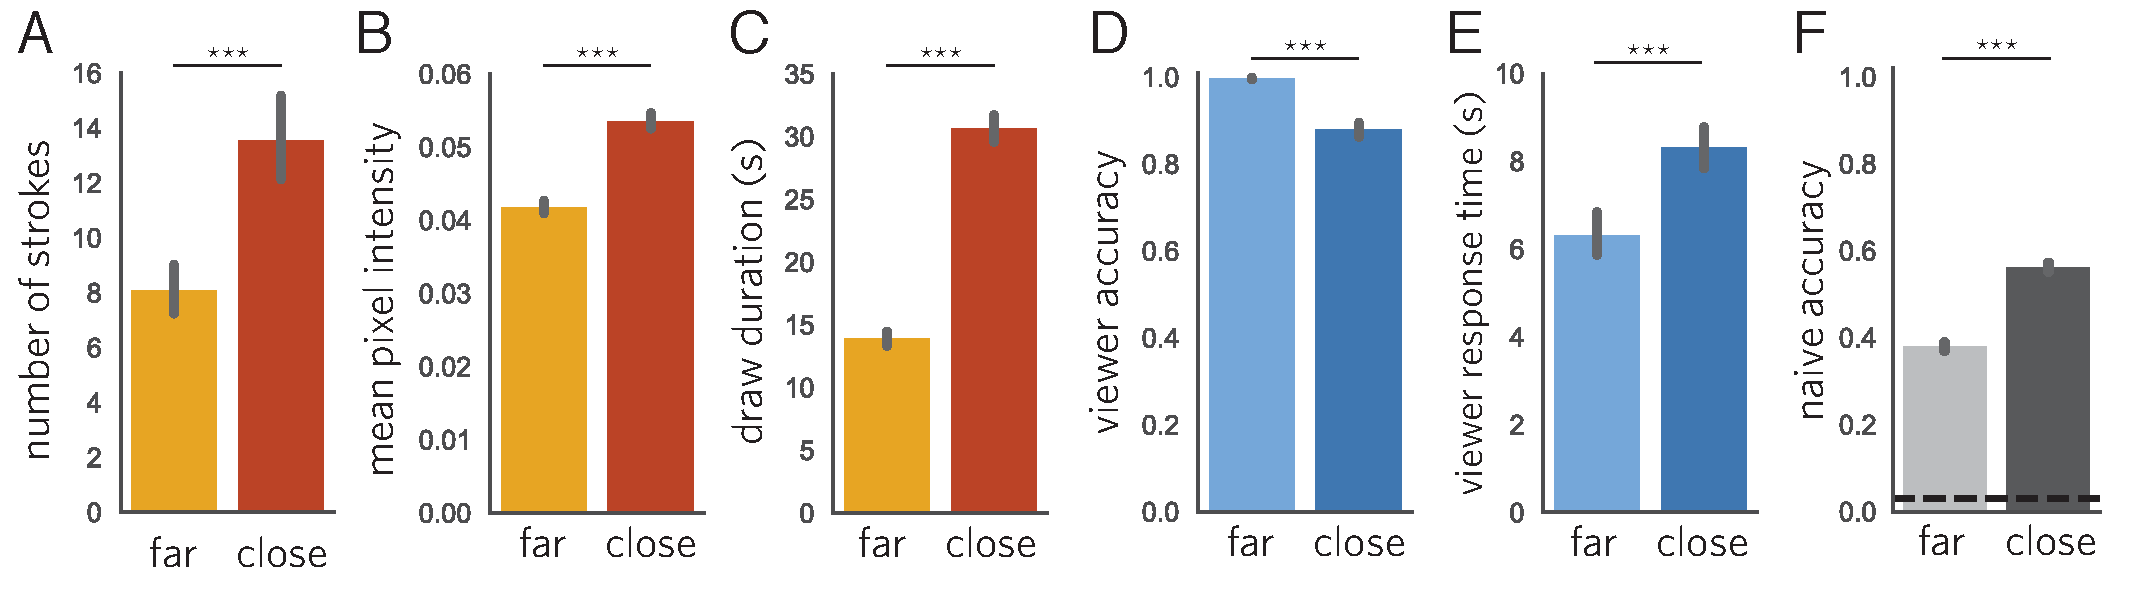
\includegraphics[width=0.9\textwidth]{figures/3_behavioral_performance.pdf}
\caption{(A-C) Mean number of strokes, amount of ink, and time spent producing sketches in each context condition. (D-E) Target identification performance in context during communication task. (F) Target identification performance out of context during recognition task.}
\label{task_performance}
\end{figure*}

%%% recognition experiments

%% Supplemental: report variation in different categories

%% Supplemental: report confusion matrix results: diagonal vs. off-diagonal block vs. rest of the matrix results.

% There was clear structure in the pattern of confusions for both close and far sketches. We further hypothesized that the particular way in which far sketches would differ perceptually from close sketches was that far sketches would be more confusable with other objects from the same basic-level category, while still being highly recognizable as a representation of the corresponding basic-level category.

% We measured this by comparing the within-category confusion rate to the overall confusion rate for close and far sketches, and found that XXX.

\subsection*{Computational model of contextual flexibility in visual communication}

Our empirical findings show that human sketchers spontaneously account for contextual information shared with the viewer, producing more informative sketches in close contexts at the cost of additional time and ink. 
Such contextual flexibility argues against the notion that sketch production is constrained exclusively by the appearance of the target of object. 
Rather, it suggests an analogy to how shared context influences what people choose to say during verbal communication, a key target of current computational theories of pragmatic language use \cite{frank2012predicting,goodman2013knowledge,franke2016probabilistic,bergen2016pragmatic}.

Informed by this work, we propose that human sketchers determine what kind of sketch to produce in context by deploying two main faculties: \textit{visual abstraction}, which refers to the ability to judge how well a sketch evokes a real object, and \textit{pragmatic inference}, which refers to the ability to judge which sketches will be sufficiently detailed to be informative about the target object in context, but no more detailed than necessary. 
% Pragmatic inference can thus be decomposed into two aspects: context sensitivity, a preference for sketches that are diagnostic of the target relative to the distractors; and cost sensitivity, a preference for sketches that require less time and effort to produce.
To test this proposal, we developed a computational model of the sketcher that embodies both visual abstraction and pragmatic inference, and was instantiated as a deep convolutional neural network nested within a probabilistic program. 
Constructing such a model allowed us to evaluate the contribution of each component using formal model comparison, as well as quantitatively characterize the model's behavior in novel contexts.
\begin{figure*}[htbp]
\centering
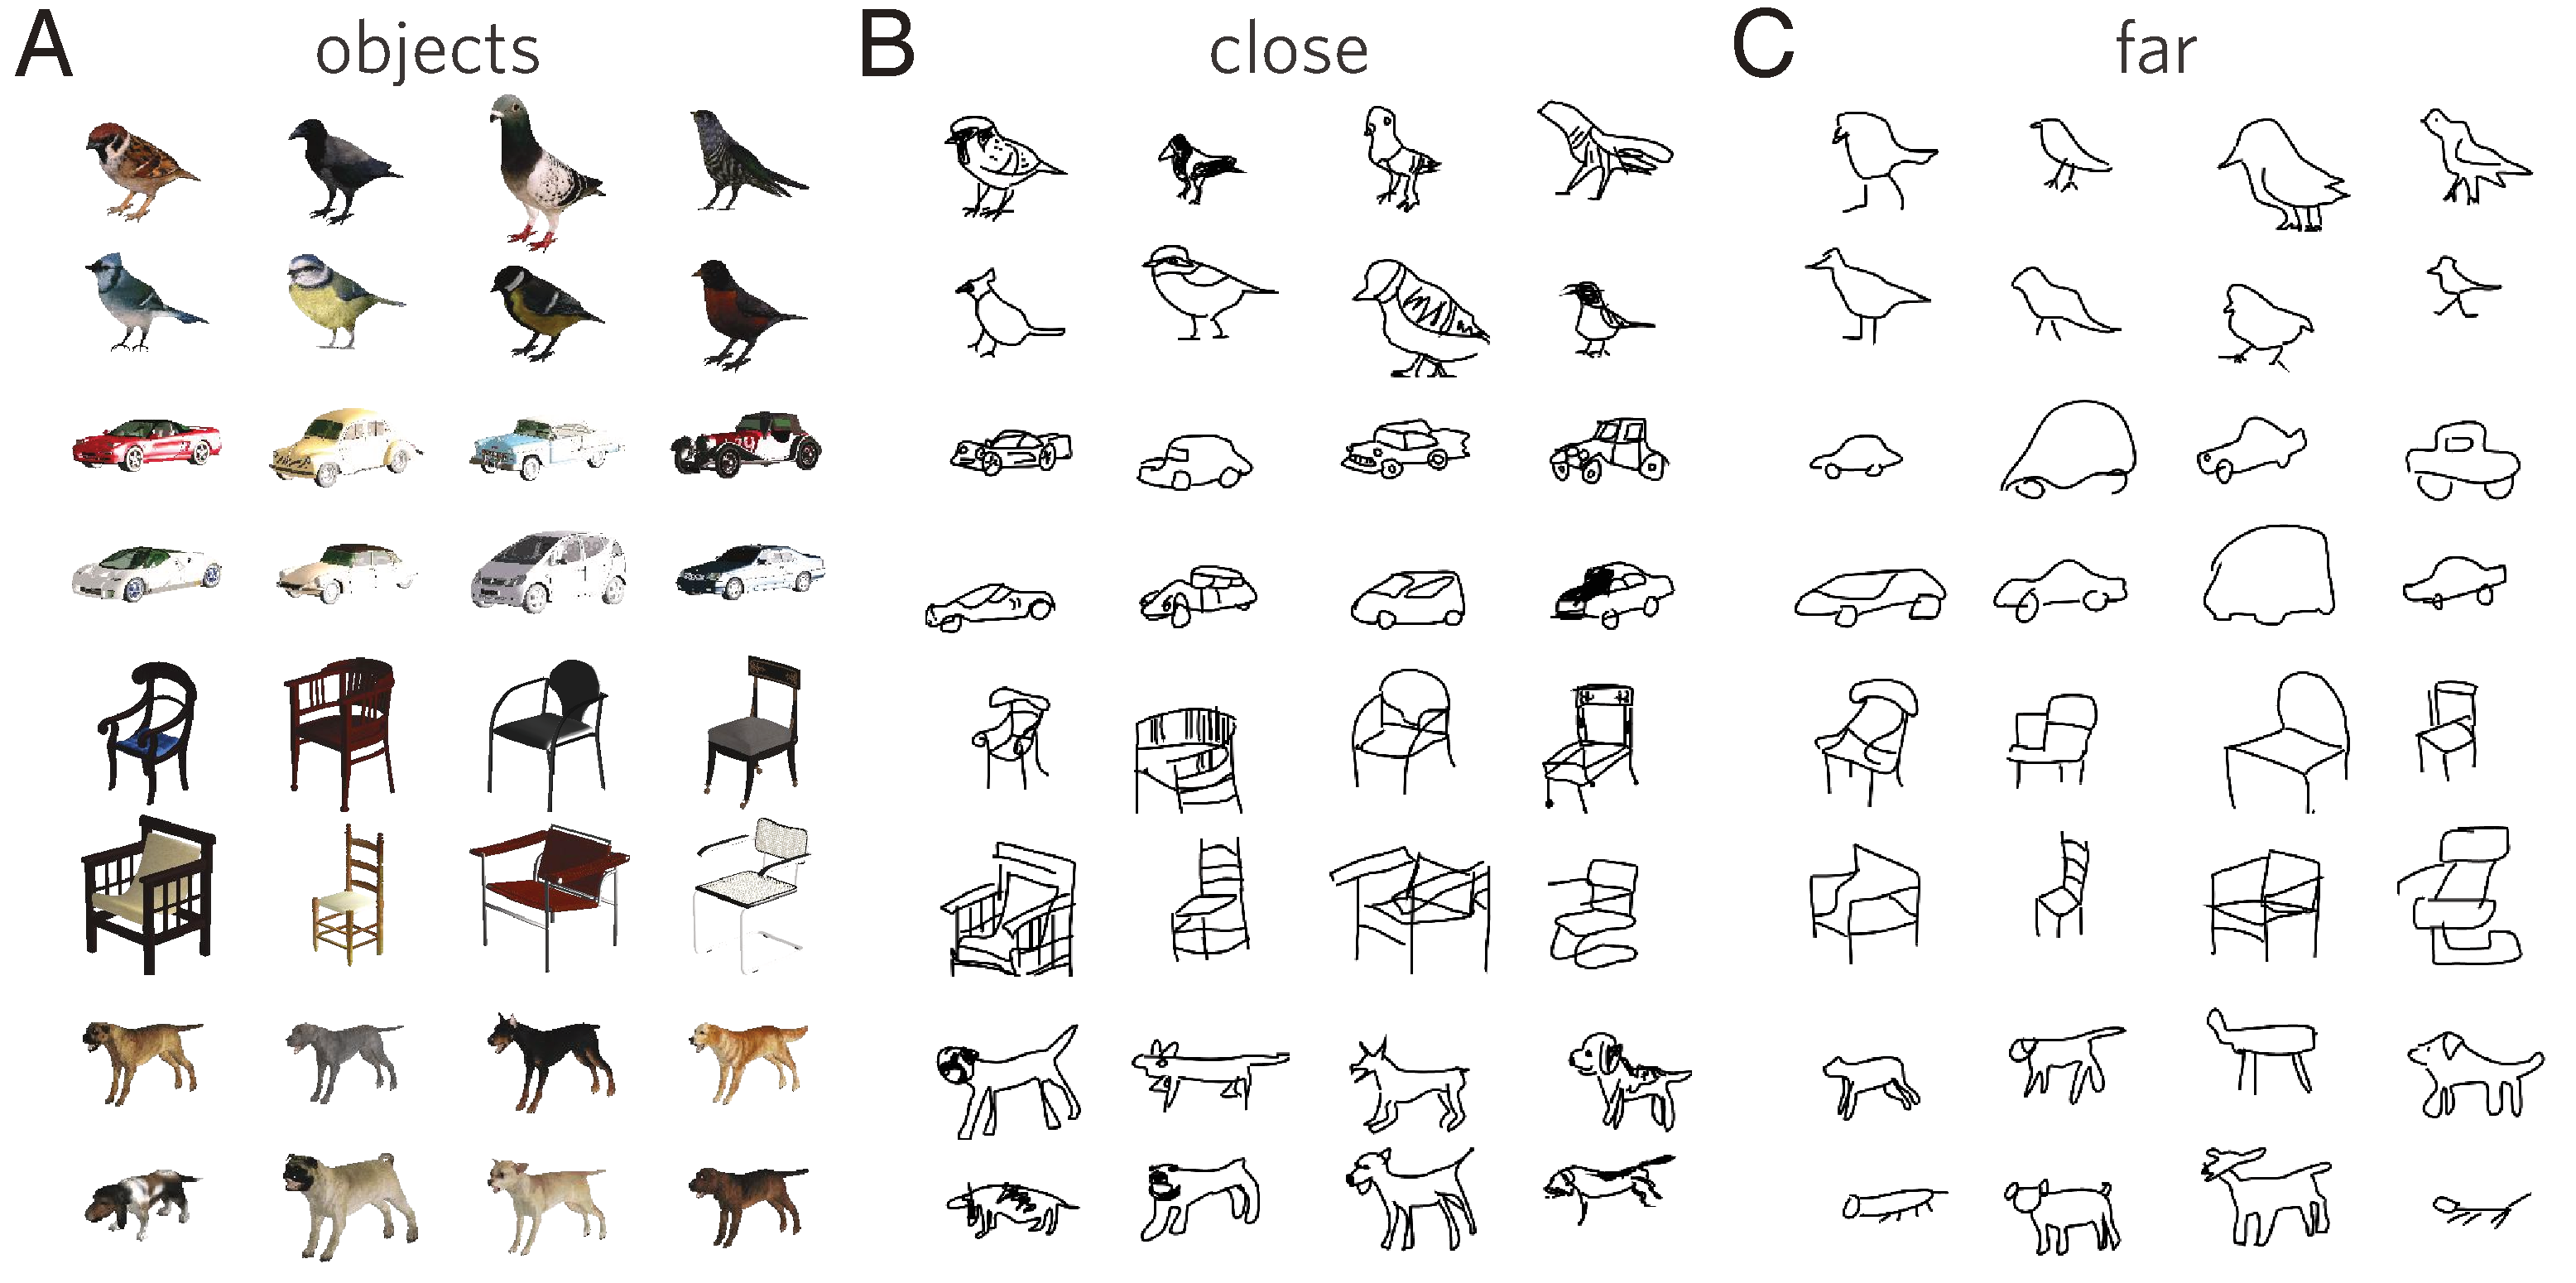
\includegraphics[width=0.9\textwidth]{figures/2_sketch_gallery-min.pdf}
\caption{(A) Object stimuli. (B) Example sketches produced in close context condition. (C) Example sketches produced in far context condition.}
\label{sketch_gallery}
\end{figure*}
\subsubsection*{Defining communicative utility of sketches}

We define a context, $O$, to be a set of objects containing a target, $t$, and three distractors,  $D=\{d_1,d_2,d_3\}$: $O = \{t,D\}$.
We define the sketcher, $\mathcal{S}$, to be a decision-theoretic agent that produces sketches of the target, $s$, proportional to their communicative utility, $U$, where the utilities of each sketch have been normalized over the set of producible sketches via the softmax function: 
\begin{equation} \label{sketcher_distribution}
\mathcal{S}(s|O) = \frac {\exp [{U(s,O)]}} {\sum_{i} {\exp [U(s_i,O)]}}
\end{equation}
In principle, the space of all producible sketches is infinite and continuous, leading to an intractable sum.
In practice, we assume that the sketcher model chooses among a large but finite set of sketches: those actually produced by participants in our experiment.

A sketcher's decision-making is determined by its utility function.
We first introduce the utility function for our proposed pragmatic sketcher, $S_{prag}$, and then consider lesioned variants for comparison. 
Overall, this utility trades off an informativity term and a cost term.
This sketcher judges a sketch's informativity to be a mixture of two quantities: one reflecting its absolute \textit{resemblance} to the target and the other its relative \textit{diagnosticity} in the presence of particular distractors (see Fig. \ref{model_schematic}B).  

Resemblance is defined by how strongly a sketch $s$ corresponds to the target $t$, i.e. $\textrm{sim}(s,t)$, which we estimate using empirical data from the recognition experiment (see Materials and Methods).
Diagnosticity is defined by the natural log probability that a simulated viewer agent, $\mathcal{V}$, would select the target object given the sketch and all objects in context, $\ln \mathcal{V}(t|s,O)$. 
The simulated viewer $\mathcal{V}$, in turn, is assumed to select the target object proportional to the correspondence between the sketch and the target, $\textrm{sim}(s,t)$, normalized by the sum of correspondences between the sketch and all four objects in context, again via the softmax function:
\begin{equation} \label{literal_viewer_score}
\mathcal{V}(t|s,O) \propto \frac {\exp\{\alpha \cdot \textrm{sim(s, t)}\}} {\sum_{i=1}^{4} \exp\{\textrm{sim}(s,o_i)\}}
\end{equation}
where $i$ indexes each object $o\in O$, and $\alpha$ is a scaling parameter determining the assumed optimality of the listener's decision policy: as $\alpha \rightarrow \infty$, the simulated viewer is more likely to choose the object with highest perceptual correspondence to the sketch. 
Intuitively, this means that the viewer is more likely to pick the correct object when the sketch corresponds more strongly to the target than to the distractors. 

To combine the resemblance and diagnosticity terms into a single informativity value, we introduce a weight parameter, $w_{d}$, that interpolates between them:
\begin{equation} \label{prag_interpolation}
I(s,O) = w_{d} \cdot \ln \mathcal{V}(t|s,O) + (1-w_{d}) \cdot \textrm{sim}(s,t). 
\end{equation} 
This captures the intuition that a communicative sketcher seeks to produce a sketch that both resembles the target object and distinguishes the target from the distractors.

Finally, we define a sketch's cost, $C(s)$, to be a monotonic function of the empirical amount of time taken to produce it, linearly transformed  to lie in the range $[0,1]$. 

Putting these terms together, we have the full utility:
\begin{equation} \label{sketcher_utility}
U_{S_{prag}}(s,O) = w_i \cdot I(s,O) - w_c \cdot  C(s)
\end{equation}
where $w_i$ and $w_c$ are independent scaling parameters that are applied to the informativity and cost terms, respectively.
These parameters determine how strongly each term contributes to the overall utility of the sketch. 
This model therefore has 4 parameters: the weights applied to informativity ($w_{i}$) and cost ($w_{c}$), the balance between diagnosticity vs.~resemblance ($w_{d}$), and the sketch-object correspondence optimality term ($\alpha$). 
We inferred these parameters from data via Bayesian data analysis (see Materials and Methods).

Within this modeling framework, we conducted a series of targeted lesion studies to test each aspect of our hypothesis about the core cognitive faculties employed by humans to decide which sketch to produce in context. 
To evaluate the necessity of pragmatics and cost, we define two simpler variants of this sketcher, which are nested within the fully pragmatic model.
A \textit{context-insensitive} sketcher, $S_{sim}$, is derived by removing the diagnosticity term from the definition of informativity (i.e.~$w_{d}{=}0$), leaving only the resemblance term. 
A \textit{cost-insensitive} sketcher, $S_{nocost}$, on the other hand, aims to produce informative sketches without regard for their cost (i.e.~$w_c=0$).
In a second set of modeling experiments, we evaluate the role of visual abstraction by using different visual features (low-level, medium-level, or high-level) for the visual correspondence \textrm{sim}(s,t).

\begin{figure*}[htbp]
\centering
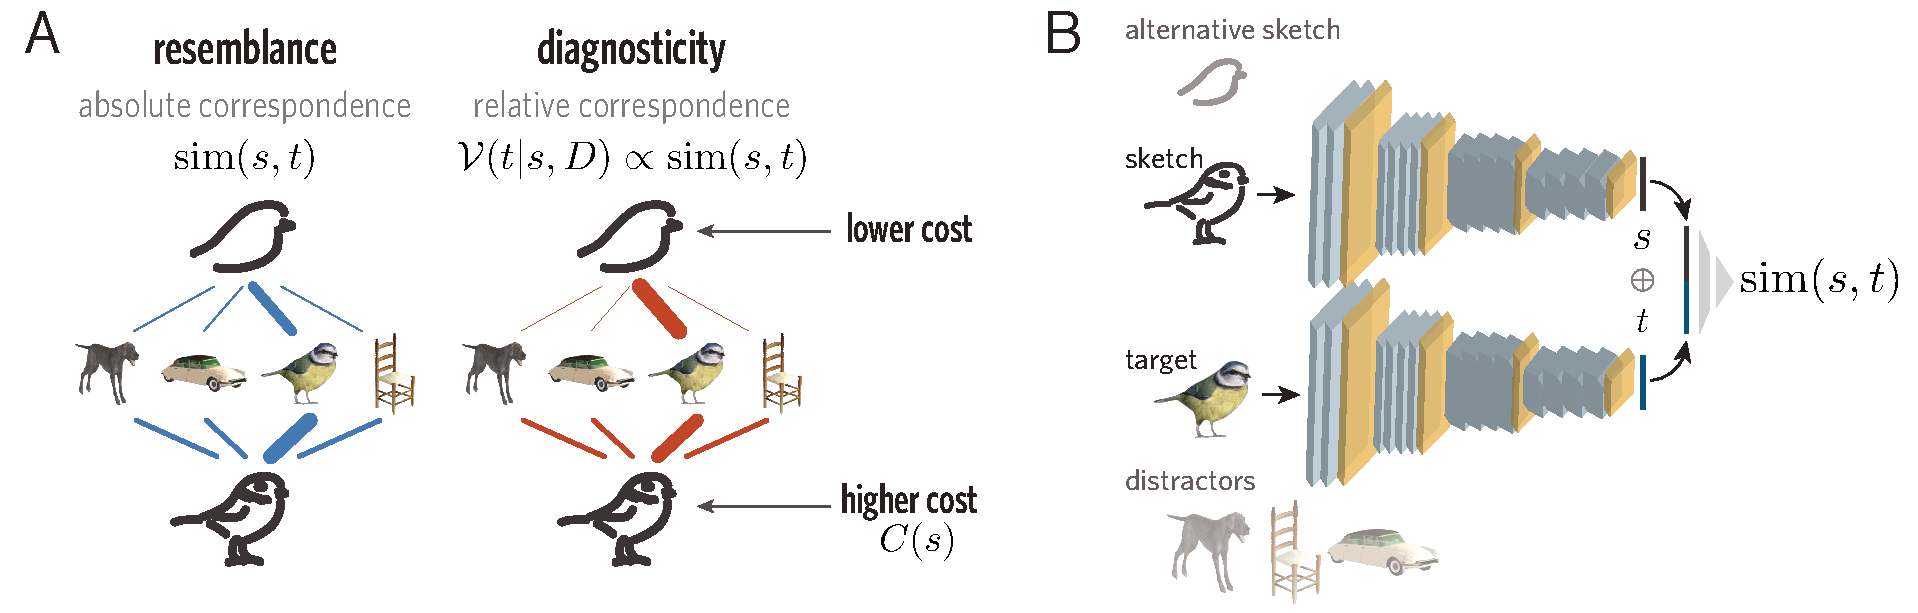
\includegraphics[width=0.95\textwidth]{figures/4_model_schematic-min.pdf}
\caption{(A) Architecture of visual encoder model for sketches and object renderings. Consists of pre-trained deep convolutional neural network (VGG-19) and shallow nonlinear ``adaptor'' neural network that predicts sketch-object correspondence. 
The encoder takes a sketch and object rendering as input, and outputs a correspondence score reflecting how well the sketch resembles the object. 
Three adaptor networks trained, using features from a one of the highest, an intermediate, and an early layer of VGG.
Each adaptor network trained and evaluated in crossvalidated fashion. 
(B) Sketch-object correspondence computed for each object in context and each sketch in the test set. 
To determine the relative informativity of each sketch, the similarity scores between this sketch and all four objects were softmax normalized. 
The cost of each sketch was assumed to vary with the amount of time taken to produce it.}
\label{model_schematic}
\end{figure*}

\subsubsection*{Evaluating contribution of pragmatic inference}

First, we evaluated the contribution of pragmatic inference by removing context sensitivity and cost sensitivity from the sketcher agent.
We hypothesized that a \textit{pragmatic} computational sketcher model that is sensitive to both context and cost would provide a strong fit to human sketch production behavior, as well as outperform lesioned alternatives lacking either component.
To test this hypothesis, we evaluated three model variants characterized by their distinct definitions of communicative utility: a pragmatic one sensitive to both context and cost ($S_{prag}$), one \textit{not} sensitive to context but sensitive to cost ($S_{sim}$), and one that \textit{is} sensitive to context but \textit{not} sensitive to cost ($S_{nocost}$).
In this set of model evaluations, we estimated the correspondence between sketches and objects, $\textrm{sim}(s,o)$ using empirical data from our recognition experiment (see Materials and Methods).

%\n_dg{we need just a few more words about how these empirical estimates are derived here or above?}
% In this and subsequent model evaluations, we defined a sketch's cost, $C(s)$, to be a monotonic function of the amount of time taken to produce it. \rdh{we said this already}

Our goal was to ascertain how well each model could produce informative sketches and appropriately modulate its behavior according to the context condition, and not necessarily to reproduce exactly the same sketch as a particular participant had on a specific trial. 
As such, we aggregated all sketches of the same object produced in the same context condition when estimating their key functional properties (i.e., perceptual correspondence, cost), so each sketch was represented by the mean in its object-context category. 
Model predictions were generated to the same level of granularity, in the form of a probability distribution over 64 types of sketches, representing each combination of object and context condition (e.g., `basset sketch produced in a close context'). 

To generate these predictions, first we employed Bayesian data analysis to infer a posterior distribution over the four latent parameters in the model ($w_{i}$, $w_{c}$, $w_{d}$, $\alpha$). 
Next, we presented each model with exactly the same set of contexts that were presented to human sketchers in the communication experiment, and evaluated the posterior predictive probabilities that each model assigned to sketches in every object-context category, marginalizing over the posterior distribution over latent parameters. 
We conduct these evaluations on each of the test sets from the same five crossvalidation folds that were used to train and test the visual encoder, to permit direct comparison of these two sets of modeling results. 

\ndg{does this mean that the posterior was fit on one fifth and then predictive evaluated on final fifth, or that posterior+predictive was on a fifth? also this is the first mention of a split into train/test folds so make it sound less like an obvious reference to something earlier?}

We found that the full model, $S_{prag}$, provided a much stronger overall fit to human behavior than the context-insensitive variant, $S_{sim}$ (median log Bayes Factor = $16.1$; see Table \ref{model_comparison}), and the cost-insensitive variant, $S_{nocost}$ (BF = $9.54$).

To explore the behavioral patterns that may explain these differences in overall performance, we examined three aspects of each model's behavior: (a) \textit{sketch retrieval}: its ability to assign a high absolute rank to the target sketch category in context, out of the 64 object-context alternatives; (b) \textit{context congruity}: its ability to consistently assign a higher rank to the context-congruent version of the target object over the context-incongruent version (i.e., on a close trial, preferring a close sketch to a far sketch); and (c) \textit{cost modulation}: how consistently it produced costlier sketches than average in the close condition, and less costly sketches than average in the far condition, mirroring human behavior.

We found that in general, sketch retrieval performance was high for all three model variants (target rank 95\% CI: pragmatic = $[1.43, 1.50]$, context-insensitive = $[1.54, 1.60]$, cost-insensitive = $[1.55, 1.60]$) (Fig.~\ref{model_results}A, left).
However, only the pragmatic sketcher was able to reliably produce the sketch appropriate for the context condition more frequently than would be predicted by chance (95\% CI proportion: $[0.571, 0.620]$; Fig.~\ref{model_results}B, left); neither the context-insensitive nor the cost-insensitive variants displayed this context congruity (95\% CI: context-insensitive = $[0.478, 0.525]$, cost-insensitive = $[0.498, 0.501]$). 
We observed that the lack of context congruity in the lesioned variants was attributable to an overall bias to produce close sketches in all contexts, which are highly informative in absolute terms, and thus higher in communicative utility if the distractors or sketch cost is ignored. 

Moreover, only the pragmatic sketcher produced costlier sketches than average in the close condition (95\% CI normalized cost: $[0.205, 0.218]$ vs. grand mean cost = $0.196$; Fig.~\ref{model_results}C, left), and less costly sketches than average in the far condition (95\%CI: $[0.175, 0.180]$). 
The context-insensitive variant is inherently unable to modulate the cost of the sketches it produces by context condition, and thus was no more or less likely to select a costlier, more diagnostic sketch on a close trial (95\% CI: $[0.187, 0.194]$) than a far trial (95\% CI: $[0.187, 0.192]$), and preferred slightly less costly sketches overall. 
While the cost-insensitive variant did exhibit cost modulation by context, because it ignores their cost, it preferred costlier sketches overall in both close (95\%CI: $[0.229, 0.241]$) and far contexts (95\%CI: $[0.214, 0.220]$). 

Together, these results suggest that both context and cost sensitivity are critical for capturing key aspects of contextual flexibility in human visual communication. 

\subsubsection*{Evaluating contribution of visual abstraction}

After establishing the importance of pragmatic inference, we next sought to evaluate the contribution of visual abstraction by comparing how features adapted from different vision models predicted human visual communication behavior. 
Having an encoding model that operates directly on image inputs is important for a computational theory of visual communication because it allows our full model to generate predictions in novel contexts (i.e., combinations of target and distractor objects).
Building on recent advances in computational vision \cite{FanCommon2018,yamins2014performance}, we instantiated the visual encoder as a deep convolutional neural network (DCNN).
This choice of model class is motivated by prior work showing that such networks, in addition to being a type of universal function approximator \cite{hornik1991approximation}, learn higher-layer feature representations that capture high-level perceptual information in drawings \cite{FanCommon2018}, capture perceptual judgments of object shape similarity \cite{kubilius2016deep}, and predict neural population responses in categories across the ventral visual stream \cite{yamins2014performance} when trained on challenging natural object recognition tasks \cite{deng2009imagenet}. 
\begin{figure*}[htbp]
\centering
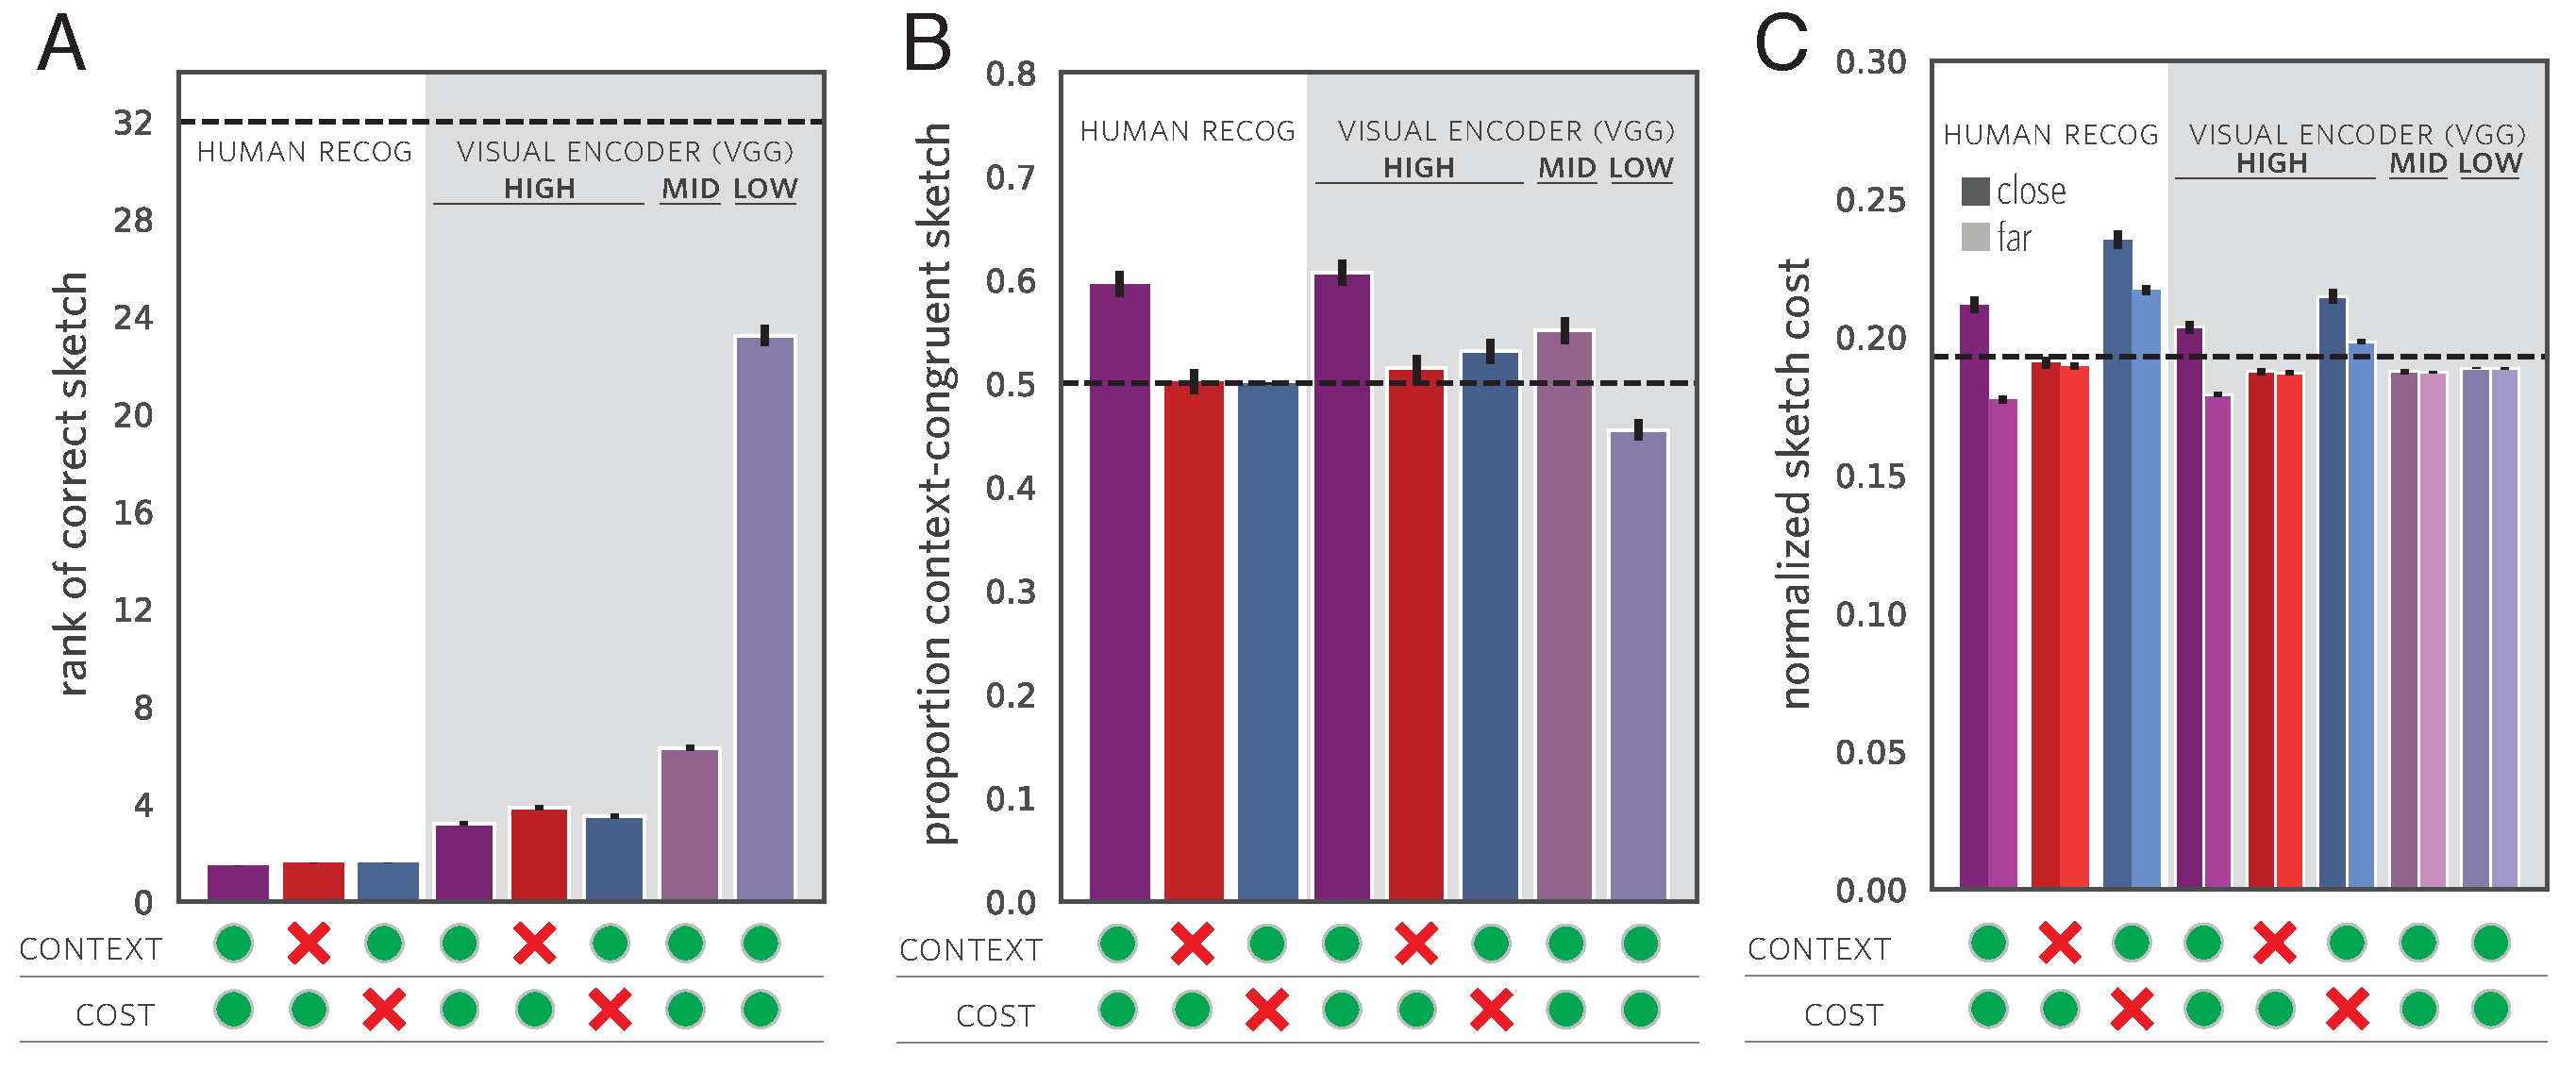
\includegraphics[width=0.99\textwidth]{figures/5_model_results_2.pdf}
\caption{Sketch production behavior by model variant. The table below each plot indicates whether the corresponding model variant plotted above is sensitive to context or cost. A green disc indicates context/cost sensitivity; a red `X' indicates the lack of context/cost sensitivity. 
Results in lefthand region of each panel (white background) reflect model predictions when using empirical estimates of $sim(s,o)$ based on human sketch recognition behavior. 
Results in the righthand region (gray background) reflect model predictions when using variants of the DCNN visual encoder, the adaptor components of which were trained in a five-fold crossvalidated manner using human sketch recognition behavior. 
All results reflect average model behavior on test data only across identical train-test splits. 
Error bars represent 1 s.e. for this average estimate, found by applying inverse-variance weighting on individual confidence intervals from each train-test split. 
A: Rank of target sketch in list of 64 object-context categories, ordered by the probability assigned by each model. 
Dashed line reflects expected target rank under uniform guessing. 
Distribution of target rank scores across models suggest that high-quality estimates of $sim(s,o)$ are critical for strong performance. 
B: Proportion of trials on which each model assigned a higher rank to the context-congruent sketch of the correct object than the context-incongruent version of the correct object. 
Dashed line reflects indifference between the two versions of the sketch. 
Only models above this line show consistent and appropriate modulation of sketch producton by context. C: Relative time cost of sketches produced by each model, after applying min-max normalization to raw draw duration measurements. 
Predicted sketch cost on each trial computed by marginalizing over probabilities assigned to each sketch category. 
Darker bars reflect behavior in the close condition; lighter bars the far condition. 
Dashed line indicates the average cost of sketches in the full dataset; bars below this line reflect a preference for sketches that are less costly than average, bars above this line for sketches that are costlier than average. 
Only models that span this dashed line match the pattern of contextual modulation of sketch cost displayed by human sketchers.}
\label{model_results}
\end{figure*}

%In order for this sketcher to generate quantitative predictions, it needs to be able to compute the perceptual correspondence, $\textrm{sim}(s,o)$, for any sketch-object pair. 
%In our second set of modeling experiments, we employ a visual encoder model adapted to predict $\textrm{sim}(s,o)$, which was trained in a crossvalidated fashion on empirical estimates of $\textrm{sim}(s,o)$.

Concretely, the visual encoder is a function that accepts a pair of images as input (see Fig. \ref{model_schematic}A): a sketch, $s$, and an object rendering, $o$, and returns a scalar value reflecting the degree of perceptual correspondence between the sketch and object, $\textrm{sim}(s,o)$, which lies in the range $[0,1]$, where $\textrm{sim}(s,o)=0$ reflects no correspondence and $\textrm{sim}(s,o)=1$ reflects maximal correspondence.
This encoder consists of two functional components: a base visual encoder network, $B$, and an adaptor network, $A$: $\textrm{sim}(s,o) = A(B(s,o))$.

% \textrm{sim}(s,o) = (\textrm{A} \circ \textrm{B}) (s,o)
We employ VGG-19 pretrained to recognize objects from the Imagenet database as our base visual encoder, whose parameters remain frozen \cite{simonyan2014very}. 
We then augment the pretrained feature representation of the base encoder with a shallow adaptor network, which is trained to predict the perceptual correspondence between specific sketch-object pairs.
We train an adaptor network because, while prior work has shown that representation of object \textit{categories} converges for sketches and photos at higher layers in DCNN models trained only on photos \cite{FanCommon2018}, additional supervision can substantially improve the accuracy of predictions involving comparisons between sketches and photos at the \textit{instance} level \cite{sangkloy2016sketchy}. 

To evaluate the importance of network depth for providing a more transferable visual feature basis for modeling human-like visual abstraction, we compare adaptor networks that intercept VGG-19 image representations at three different layers: the first max pooling layer (early), the tenth convolutional layer (mid), and the first fully connected layer (high).
Critically, all adaptor networks contained approximately the same number of learnable parameters, and were trained on the same data using exactly the same optimization procedure for an equal number of epochs. 
All model evaluations involving the base encoder and trained adaptor network were performed in a fivefold crossvalidated manner, with the full communication task dataset split into training, validation, and test sets in a 80\%, 10\%, and 10\% ratio.
We followed the same procedure as above to generate model predictions for the test set of each crossvalidation fold of our dataset, such that each visual encoder was trained on a different subset of the data than was used to evaluate it. 

% \n_dg{one more sentence about the data / training of the adaptor would be useful here.}
% \mikewu{this might not be important for this paper, but actually pretty interesting that we need nonlinearities in the adaptation, meaning that the spaces are not aligned in an affine sense... these two sentences about (1) we can generalize to sketches out of the box, and (2) we need additional transformations seem contradictory. How do we explain this? @jefan: I think it's probably not too different from the way for most visual transfer learning problems, we usually need to learn some nonlinearities to get good performance on the transfer task. But Imagenet-training being prety reasonable as a place to start is a pretty consistent pattern, even leaving aside sketch reprsentation. }
% Consistent with prior work \cite{kubilius2016deep,FanCommon2018}, 
%To explore the degree to which the visual abstraction afforded by the complex transformations applied by successive layers of VGG-19 are required to capture human behavior during visual communication, we hypothesized that 
%higher layers of these networks would provide a more transferable visual feature basis for modeling human-like visual abstraction in this task, relative to the lower-level image statistics represented in earlier layers.
% Motivated by other prior work suggesting that higher-level visual features provide a better fit to human perceptual judgments than features from earlier layers \cite{kubilius2016deep}, we hypothesized that generalization to novel communication contexts would be supported by a visual encoder that uses high-level features to predict sketch-object correspondences, rather than lower-level features from earlier or intermediate layers of the neural network.
%\n_dg{it feels like there should be a section heading here? otherwise move this paragraph to start of next subsection?}

Consistent with our hypothesis, we found that a pragmatic sketcher model employing high-level features provided a substantially better fit to the data than one using mid-level features (high vs. mid median BF: $94.8$) or low-level features (high vs. low BF: $257$). 
These results show that making fuller use of the depth of VGG to compute the perceptual correspondence between a sketch and object yields a stronger basis for explaining human visual communication behavior.

Critically, using high-level features supported strong performance on sketch retrieval (95\% CI target rank: $[3.03, 3.37]$, Fig.~\ref{model_results}A), compared to mid-level features (target rank: $[6.05, 6.56]$) and low-level features (target rank: $[22.4, 24.1]$). 
These results show that without a high-performing visual encoder, the model is much less likely to produce sketches of the correct object, a basic prerequisite for successful visual communication even in the absence of contextual variability. 

Moreover, the pragmatic sketcher model using high-level features also displayed context congruity (95\% CI: $[0.583, 0.632]$, Fig.~\ref{model_results}B), comparable in degree to the best-performing pragmatic model that lacked an encoder, showing that our full sketcher model was able to successfully reproduce this key signature of contextual flexibility for novel communicative contexts and sketches. 
The variant using mid-level features also displayed context congruity to a weaker extent (95\% CI: $[0.526, 0.576]$), suggesting that an intermediate level of visual abstraction could achieve an intermediate degree of context congruity. 
By contrast, the variant using low-level features failed to prefer the context-congruent sketch category (95\% CI: $[0.435, 0.475]$), providing a lower bound on the level of visual abstraction required in the underlying vision model to support flexible visual communication behavior. 

Again, only the pragmatic sketcher model using high-level features displayed the same pattern of cost modulation as the best-performing pragmatic model lacking an encoder (95\%CI: close = $[0.199, 0.208]$, far = $[0.178, 0.181]$, Fig.~\ref{model_results}C), while both of the other variants using mid-level and low-level features failed to do so (95\%CI: mid-level: close = $[0.186, 0.189]$, far = $[0.186, 0.188]$; low-level: close = $[0.188, 0.189]$, far = $[0.188, 0.189]$).  

Having identified the best-performing visual encoder as the one that adapted features from a higher layer of VGG, we then performed the same context and cost sensitivity lesion experiments as before in order to evaluate the contribution of pragmatic inference in our full model. 
Again, we found that the pragmatic sketcher provided a stronger overall fit to human behavior than the context-insensitive variant (median Bayes Factor = $28.1$; see Table \ref{model_comparison}), and a modestly better fit than the cost-insensitive variant (BF = $1.98$). 
% \mikewu{do we have intuition as to why this one is only modestly better?}
Critically, we found that removing context and cost sensitivity diminished the ability of this model to produce the context-congruent sketch of the correct object (context-insensitive 95\% CI: $[0.489, 0.539]$; cost-insensitive 95\% CI: $[0.507, 0.554]$; Fig.~\ref{model_results}B), and appropriately modulate the cost of the sketches it produced (context-insensitive 95\% CI: close = $[0.185, 0.190]$, far = $[0.185, 0.189]$; cost-insensitive 95\% CI: close = $[0.210, 0.219]$, far = $[0.196, 0.200]$; Fig.~\ref{model_results}C). 
By contrast, these lesions led to only modest decrements in overall sketch retrieval performance (95\% CI target rank: context-insensitive = $[3.65, 4.05]$, cost-insensitive = $[3.33, 3.67]$;  Fig.~\ref{model_results}A), suggesting that the visual encoder itself is a major determinant of the ability to produce sketches of the correct \textit{object}, even if not the context-congruent version.
These results converge with those of the lesion experiments conducted on the pragmatic sketcher model without a visual encoder, and together provide strong evidence for the importance of both visual abstraction and pragmatic inference for explaining contextual flexibility in human visual communication. 

\ndg{i think we need some direct comparison of full model with and without encoder.... without encoder will win, and then we point out that it doesn't provide an explanation of the visual aspect as the encoder one does?}

\begin{table*}[]
\centering
\begin{tabular}{@{}lll|llll@{}}
\toprule
\multicolumn{1}{{c}}{} & \multicolumn{2}{c|}{\textbf{human recog}} & \multicolumn{4}{c}{\textbf{visual encoder}} \\ \midrule
\multicolumn{1}{c}{\textbf{split}} & \multicolumn{1}{c}{\textbf{context vs. no-context}} & \multicolumn{1}{c|}{\textbf{cost vs. no-cost}} & \multicolumn{1}{c}{\textbf{context vs. no-context}} & \multicolumn{1}{c}{\textbf{cost vs. no-cost}} & \multicolumn{1}{c}{\textbf{high vs. mid}} & \multicolumn{1}{c}{\textbf{high vs. low}} \\
\textbf{1} & 18.0 & 11.9 & 44.5 & 2.70 & 105 & 282 \\
\textbf{2} & 8.46 & 9.89 & 20.9 & -0.33 & 92.5 & 242 \\
\textbf{3} & 19.2 & 8.95 & 31.9 & 1.98 & 94.8 & 257 \\
\textbf{4} & 13.4 & 9.54 & 8.35 & -0.67 & 93.4 & 248 \\
\textbf{5} & 16.1 & 7.92 & 28.1 & 5.99 & 114 & 269 \\
\textbf{median} & \textbf{16.1} & \textbf{9.54} & \textbf{28.1} & \textbf{1.98} & \textbf{94.8} & \textbf{257} \\ \bottomrule
\end{tabular}
\caption{Log Bayes Factors (BF) for comparisons between full and lesioned model variants (columns) for each crossvalidation fold (rows). 
Log-BFs$>$0 indicate greater evidence for the full model than the lesioned variant. 
Human Recog: used empirical estimates of perceptual correspondence based on human sketch recognition behavior. 
Visual Encoder: used DCNN visual encoder, trained in a five-fold crossvalidated manner using human sketch recognition behavior. 
Context: comparison between context-sensitive and context-insensitive variant. 
Cost: comparison between cost-sensitive and cost-insensitive variant; 
Mid: comparison between high adaptor vs. mid adaptor in context/cost-sensitive model; 
Low: comparison between high adaptor vs. low adaptor in context/cost-sensitive model.}
\label{model_comparison}
\end{table*}


%%%%%%%% cost fc6, context fc6, high vs. mid, high vs. low, cost human, context human
% 	1 & 2.70 & 44.54 & 105.51 & 281.65 & 11.93 & 17.98 \\ 
%   2 & -0.33 & 20.93 & 92.45 & 241.84 & 9.89 & 8.46 \\ 
%   3 & 1.98 & 31.86 & 94.77 & 256.83 & 8.95 & 19.15 \\ 
%   4 & -0.67 & 8.35 & 93.41 & 247.57 & 9.54 & 13.41 \\ 
%   5 & 5.99 & 28.12 & 113.59 & 268.80 & 7.92 & 16.07 \\ 
%   median & 1.98 & 28.12 & 94.77 & 256.83 & 9.54 & 16.07 \\ 
%%%%%%%% cost fc6, context fc6, high vs. mid, high vs. low, cost human, context human

\section*{Discussion}

The present study examined how communicative context influences visual communication behavior in a sketching-based reference game. 
We explored the hypothesis that people spontaneously account for information in common ground with their communication partner to produce drawings that are diagnostic of the target relative to the alternatives, while not being too costly to produce. 
We found that people spontaneously modulate how much time they invest in their drawings according to how similar the distractors are to the target, spending more time to produce more informative drawings when the alternatives were highly similar, but getting away with spending less time and producing less informative drawings when the alternatives were highly distinct.
Observing such contextual flexibility suggests that while visual abstraction --- the capacity to perceive the correspondence between an object and a drawing of it --- is important for explaining why drawings of objects look the way they do, visual production is not constrained exclusively by the perceptual properties of an object.  
Rather, our findings exposed an additional role for pragmatic inference --- the ability to infer what information would be \textit{relevant} to communicate, and not merely true.
To test this hypothesis, we developed a computational model that embodied both pragmatic inference and visual abstraction, and found that it predicted human communication behavior well, and outperformed variants of the model lacking either component. 
Together, this paper provides a first algorithmically explicit theory of how perceptual and social cognition support contextual flexibility during visual communication.

% related literatures
% relationship to RSA models to language
This work generalizes the Rational Speech Act (RSA) modeling framework, originally developed to explain contextual effects in verbal communication \cite{frank2012predicting,goodman2013knowledge,franke2016probabilistic,bergen2016pragmatic}, to the domain of visual communication.
RSA models take inspiration from the insights of Paul Grice \cite{grice1975syntax}, and incorporate ideas from decision theory, probabilistic models of cognition, bounded rationality, and linguistics, to understand how substantial variance in natural language use can be explained by general principles of social cognition. 
They have been shown to capture key patterns of natural language use \cite{goodman2013knowledge}, achieve good quantitative fits with experimental data \cite{kao2014formalizing}, and enhance the ability of artificial agents to produce informative language in reference game tasks \cite{monroe2017colors,Cohn-GordonGP18}.
In successfully adapting this modeling approach to the visual domain, our findings provide novel evidence for the possibility that similar cognitive mechanisms may underlie pragmatic behavior in both verbal and nonverbal communication modalities, a notion implicitly endorsed by prior work that has used nonverbal modalities (e.g., sketching, gesture) to investigate functional constraints on communication shared with language
\cite{goldin1977development,Garrod:2007wk,fay2010interactive,theisen2010systematicity,garrod2010can,Galantucci:2005uh,verhoef2014emergence}. % mention that prior studies haven't manipulated context? 
Moreover, they provide a principled strategy for understanding how variability across depictions of the same object can be derived from the task goals of the sketcher --- in this case, to coordinate with a viewer on the same object of reference in context. 
 % --- in this case, to coordinate with a viewer on the same object of reference in a context with mutually known alternatives.
In particular, future work exploring the joint consideration of communicative goals and perceptual representation during visual communication may help to provide mechanistic insight into the emergence of graphical conventions among communicators who build up common ground across repeated interactions. 

% limitations of this work
	% requires heavy supervision to get adaptor to work well, suggests that we need better approach to approximating image-level correspondence
	% greater diversity in shapes and contexts
	% image-level predictions

% future directions
	% pix2svg -- fully generative model that produces strokes
	% graphical conventions 
	% neural mechanisms of contextual flexibility
	% better characterization of the subsetting/smoothing that characterizes visual abstraction	

There are several limitations of our model that would be fruitful to address in future work. 
First, obtaining a visual encoder that could produce accurate predictions of perceptual correspondence between sketch-object pairs required substantial supervision. 
While heavy supervision is not uncommon when developing neural network models of sketch representation \cite{sangkloy2016sketchy,yu2017sketch,song2017deep}, future work should investigate architectures that require weaker supervision to estimate image-level correspondences between sketches and natural photographs. 
One promising approach may be to exploit the hierarchical and compositional structure of natural objects (i.e., parts, subparts, and their relations), as they are expressed in both natural images and sketches of objects \cite{battaglia2016interaction,mrowca2018graph}.
Second, our model produces a decision over which \textit{type} of sketch to produce in context, rather than producing a \textit{particular} sketch.  
This is of course different from the action selection problem human participants face --- they must decide not only what stroke to make, but where to place them, how many, and in what order.
While there have been recent and promising advances in modeling sketch production as a sequence of such actions \cite{lake2015human,ha2017neural,ganin2018synthesizing}, these approaches have not yet been shown to successfully emulate how people sketch real objects, much less how this behavior is modulated by communicative context. 
Future work should develop sketch production models that both operate on natural visual inputs and more closely approximates the the action space inherent to the task.
Meeting these challenges is not only important for developing more human-like artificial intelligence, but may also shed new light on the nature of human visual abstraction, and how online perception and long-term conceptual knowledge guide decision making during complex, natural behaviors. 

In the long term, investigating the computational basis of visual communication may help to elucidate the sources of cultural variation in pictorial style, reveal the origins of modern graphical techniques for conveying patterns in data, and lead to enhanced interactive visualization tools for education and research.

\subsubsection*{Code availability} The code for the analyses presented in this article is publicly available in a Github repository at: \url{https://github.com/judithfan/visual_communication_in_context}.

\subsubsection*{Data availability} The data presented in this article are publicly available in a figshare repository.

% \subsection*{Supporting Information (SI)}

% The main text of the paper must stand on its own without the SI. Refer to SI in the manuscript at an appropriate point in the text. Number supporting figures and tables starting with S1, S2, etc. Authors are limited to no more than 10 SI files, not including movie files. Authors who place detailed materials and methods in SI must provide sufficient detail in the main text methods to enable a reader to follow the logic of the procedures and results and also must reference the online methods. If a paper is fundamentally a study of a new method or technique, then the methods must be described completely in the main text. Because PNAS edits SI and composes it into a single PDF, authors must provide the following file formats only.

\matmethods{

\subsection*{Communication experiment: Manipulation of context in sketch-based reference game}

\subsubsection*{Participants}
A total of 192 unique participants, who were recruited via Amazon Mechanical Turk (AMT) and grouped into pairs, completed the experiment. 
They were provided a base compensation of \$2.70 for participation and earned a \$0.03 bonus for each correct trial. 
In this and subsequent behavioral experiments, participants provided informed consent in accordance with the Stanford IRB.
\subsubsection*{Stimuli and Task}
Because our goal was to understand how context influences how much detail people use to distinguish objects from one another during visual communication, we populated our reference game with contexts possessing two key properties: (1) they contained familiar real-world objects, so that a primary source of variation would be driven by context, rather than difficulty recognizing or sketching the objects, \textit{per se}; and (2) they systematically varied in target-distractor similarity within a session, lending greater statistical power to comparisons between context conditions. 
To achieve these objectives, we obtained thirty-two 3D mesh models of objects belonging to 4 basic-level categories (i.e., birds, chairs, cars, dogs), containing eight objects each. 
Each object was rendered in color on a gray background at three-quarter perspective, 10$^{\circ}$ viewing angle (i.e., slightly above), and fixed distance. 
Independently in each experimental session, objects were allocated to eight sets of four objects: Four of these sets contained objects from the same category (``close''); the other four of these sets contained objects from different categories (``far'' condition).
The assignment of objects to set and condition was randomized across pairs.
Each set of four objects was presented four times each, such that each object in the quartet served as the target exactly once. 

% \subsubsection*{Task}
% Drawings were collected in the context of an online, sketching-based reference game (``Guess My Sketch!''). The game involved two players: a \textit{sketcher} who aims to help a \textit{viewer} pick out a target object from a set of distractor objects by representing it in a sketch. On each trial, both participants were shown an array of the same four objects; however, the positions of these objects were randomized for each participant so that participants could not use object location information to solve the task. On each trial, one of the four objects was highlighted on the sketcher's screen to designate it as the target.
Sketchers drew using black ink on digital canvas (pen width = 5 pixels; 300 x 300 pixels) embedded in a web browser window using Paper.js (http://paperjs.org/). Participants drew using the mouse cursor, and were not able to delete previous strokes. Each stroke of which was rendered on the viewer's screen immediately upon the completion of each stroke. There were no restrictions on how long participants could take to make their drawings. After clicking a submit button, the viewer guessed the identity of the drawn object by clicking one of the four objects in the array. Otherwise, the viewer had no other means of communicating with the sketcher. Both participants received immediate task-related feedback: the sketcher learned which object the viewer had clicked, and the viewer learned the identity of the target. Both participants earned bonus points for each correct response.

% Successful communication was primarily quantified as the viewer's accuracy in identifying the target. The investment of time was measured as the length of time between the beginning of the first stroke to the completion of the final stroke in each sketch, and the investment of ink was measured in two ways: as the number of strokes used for each sketch and the proportion of the drawing canvas filled by ink.

\subsection*{Recognition experiment: Measuring perceptual similarity between sketches and objects}

\subsubsection*{Participants}

A total of 112 participants were recruited via Amazon Mechanical Turk (AMT). They were provided a base compensation of \$1.00 for their participation, and earned an additional \$0.01 bonus for each correct response.

\subsubsection*{Task}
On each trial, participants were presented with a randomly selected sketch collected in the communication experiment, surrounded by a grid containing the 32 objects from that experiment. 
Their goal was to select the object in the grid that best matched the sketch. 
% Participants were provided with binary feedback about the correctness of their response on each trial via a bonus counter that incremented by 1 point for each correct identification, but did not change for incorrect trials. 
Participants received task feedback in the form of a bonus earned for each correct trial. 
Participants were instructed to prioritize accuracy over speed. 
We applied a conservative outlier removal procedure based on response latency, whereby trials that were either too fast to have supported careful consideration of the sketch and menu of objects (RT<$1000ms$), or too slow and suggestive of an attentional lapse (RT>$30s$), were filtered from the dataset. 
The removal of these outlier trials ($8.01$\%) did not have a substantial impact on the pattern of recognition behavior. 
In order to mitigate the possibility that participants could adjust their matching strategy according to any particular sketcher's style, each session was populated with 64 sketches sampled randomly from different reference games. 
To obtain robust estimates of sketch-object perceptual correspondences, each sketch was presented approximately 10 times across different sessions.  

% VERIFY THIS: Participants were permitted to complete multiple sessions of this task, but were prevented from providing identification judgments for the same sketch twice, or for sketches they themselves had produced or viewed (on the rare occasion that this participant had also participated in the reference game experiment).

\subsection*{Computational modeling}

% We hypothesized that two core cognitive faculties are necessary and sufficient for explaining contextual flexibility in the visual communication task: (1) visual abstraction, the capacity to perceive the high-level perceptual correspondence between an object and a drawing of it; and (2) pragmatic inference, the ability to infer what information would help a viewer distinguish the target from distractors.

% To test this proposal, we developed a computational model of the sketcher that embodied both visual abstraction and pragmatic inference, and was instantiated as a probabilistic program ``wrapped'' around a deep convolutional neural network. 
% Constructing such a model allowed us to evaluate the contribution of each component using formal model comparison, as well as quantitatively characterize the model's behavior in novel contexts. 

\subsubsection*{Sketch data preprocessing} 
To train and evaluate our sketcher model, we first filter the sketch dataset to retain only sketches that were correctly identified by the viewer during the communication task (6.2\% incorrect) and were compliant with task instructions by not including `drawn' text annotations (4.4\% non-compliant). 
% Only correctly identified sketches were retained to mitigate the amount of noise in estimating sketch-object correspondences
% and to simplify the interpretation of the model likelihood: we score each model according to the probability it assigned to the ground truth sketch category, which we assume to have led to successful communication. 
This filtered sketch dataset was then split into training, validation, and test sets in a 80\%, 10\%, and 10\% ratio, and this split was performed in a 5-fold cross-validated manner.
Splits were based on context, defined as the set containing a specific target object and three distractor objects, such that no context appeared both in the training and test splits of any cross-validation fold. 
Specifically, we ensured that: (1) the number of sketches from each category (i.e. car) and (2) the proportion of sketches from close and far trials were equated across splits. 
This was done to control for biases in model peformance due to imbalances in the training or test set.

\subsubsection*{Deriving empirical estimates of perceptual correspondence between sketches and objects}

% We evaluate our model using both empirical and model-based approaches to measuring perceptual correspondence. 
In the recognition experiment, most sketches were not matched exclusively to a single object, but to several. 
These sketches can thus be thought of having some degree of perceptual correspondence to the several objects it was matched to at least once. 
For a single sketch, we estimate the perceptual correspondence between that sketch and any object as the proportion of recognition task trials on which it was matched to that object. 
For a set of sketches of a specific object produced in a specific context condition, we estimate the \textit{aggregated} sketch-object correspondence to be the proportion of recognition task trials on which any sketch from this set was matched to that object. 
Because our goal was to understand how well each model could produce produce informative sketches according to the context condition, and not necessarily to reproduce exactly the same sketch as a particular participant had on a specific trial, we use this aggregate correspondence measure in all of our modeling experiments.  
As a result, sketch-object correspondence scores lie in the range $[0,1]$, and sum to 1 for sketches in the same object-context category. 
Because all sketches from the same object-context category share the same correspondence to each object, there are a total of 32 sketch categories x 32 objects x 2 contexts = 2048 empirical perceptual correspondence scores.



% $\sum_{n=1}^{32} \textrm{sim} (s,o_{n}) = 1$, where $n$ is over the 32 objects in our stimulus set, $s$ refers to all sketches from the same object-context category. 
% Model-based perceptual correspondence scores are defined to the same level of granularity, with all sketches from the same object-context category sharing the same perceptual correspondence to a particular object, under a particular choice of visual encoder module (i.e., vgg-high, vgg-mid, vgg-low).



\subsubsection*{Deriving empirical estimates of sketch costs}

% While we are presently agnostic to the underlying representation of sketch cost used by participants, we assumed the cost of each sketch to be proportional to the amount of time taken by the participant to produce it during the communication task. 
We reasoned that drawing time would be a natural proxy for the cost incurred by workers on Amazon Mechanical Turk, who increase their total compensation by completing tasks in a timely manner. 
However, as there were no absolute constraints on the amount of time that could be spent on each trial, there was considerable variability across different participants in terms of how much time they spent producing their sketches. 
To control for this variability across participants and to ensure robust estimates, we first removed outliers (draw times exceeding 5 s.d. from the mean), then z-score normalized drawing times across all remaining trials within a participant, and finally averaged these normalized draw times across sketches within the same object-context category as above, yielding 32 objects x 2 contexts = 64 empirical cost estimates in total.

\subsubsection*{Visual encoder architecture}

The visual encoder is a function that accepts a pair of images (both 224 x 224 RGB), a sketch and an object rendering, as input and returns a scalar value in the range $[0,1]$, reflecting the degree of perceptual correspondence between the sketch and object. 

The encoder consists of two components: a base visual encoder and an adaptor network. 
We employed VGG-19 \cite{simonyan2014very} as our base visual encoder architecture.
We augmented VGG-19 with a shallow fully-connected \textit{adaptor} network that is trained predict the perceptual correspondence between individual sketch-objecet pairs. 
Here only the parameters of this adaptor network are trained and we do not finetune the base visual encoder. 
We compared three adaptor networks that intercept VGG-19 image representations at different layers: the first max pooling layer (early), the tenth convolutional layer (mid), and the first fully connected layer (high). 
To facilitate comparison between adaptor networks, we ensured that each of the three contain a comparable number of trainable parameters (number of learnable parameters for high: $1048839$; mid: $1049115$; low: $1048833$) with identical training hyperparameters (i.e., learning rate, batch size, etc.). 
To discriminate which layer provides the best starting feature basis for predicting sketch-object correspondence, these adaptor networks were also deliberately constrained to be shallow, i.e., consisting only of two linear layers with an intervening point-wise nonlinearity.

\textbf{High.} When applying the high-level visual encoder, a sketch and object were first passed through VGG and a feature vector in $\mathbb{R}^{4096}$ for each image is extracted from the one of the highest layers (i.e., the first fully-connected layer, also known as \textit{fc6}). 
These two vectors were then concatenated to form a single vector in $\mathbb{R}^{8192}$, to be passed into the high adaptor network. 
The high adaptor is composed of one linear layer that maps from $\mathbb{R}^{8192} \rightarrow \mathbb{R}^{128}$, followed by a ``Swish'' nonlinearity \cite{ramachandran2018searching} and dropout, then a second linear layer mapping from $\mathbb{R}^{128} \rightarrow \mathbb{R}^{1}$.
Swish is a recently discovered nonlinearity that outperforms the common rectified linear nonlinearity (ReLU) in deep models on several benchmarks \cite{ramachandran2018searching}.
Dropout was applied to mitigate overfitting and improve generalization \cite{hinton2012improving,gal2015dropout}.

\textbf{Mid.} When applying the mid-level visual encoder, sketch and object representations are intercepted from an intermediate layer (i.e., the 10th convolutional layer, \textit{conv\_4\_2}).
Features in this layer are of dimensionality 512 x 28 x 28.
Each of the sketch and object feature tensors were then ``flattened'' to a one dimensional vector in $\mathbb{R}^{512}$ using a weighted linear combination over the spatial dimensions $\sum_{i=1}^{28}\sum_{j=1}^{28} w_{ij} * x_{ij}$, where $x_{ij}$ indexes a spatial location in the image representation at this layer (i.e., `soft attention' over the spatial dimension, \cite{xu2015show}). 
These weights $\{w_{ij}|1\leq i,j \leq 28\}$ are learned jointly with the parameters of the rest of the mid adaptor, but learned independently between sketch and object image modalities \cite{xu2015show}. 

The two feature vectors in $\mathbb{R}^{512}$ are then concatenated to form a single vector in $\mathbb{R}^{1024}$.
Following the architecture of the high adaptor, the mid adaptor consists of a linear layer that maps from $\mathbb{R}^{1024} \rightarrow \mathbb{R}^{1021}$, followed by a Swish nonlinearity, dropout, then a linear layer from $\mathbb{R}^{1021} \rightarrow \mathbb{R}^{1}$. 

\textbf{Low.} When applying the low-level visual encoder, sketch and object representations are intercepted from the first max pooling layer (i.e., \textit{pool1}).
Features in this layer are of dimensionality 64 by 112 by 112. 
As above, a weighted sum of model activations over the spatial dimension was applied first (112 x 112), yielding a sketch and object vector, both in $\mathbb{R}^{64}$, which were then concatenated to form a single vector in $\mathbb{R}^{128}$. 
This was followed by a linear layer that maps from $\mathbb{R}^{128} \rightarrow \mathbb{R}^{7875}$, then a Swish nonlinearity, dropout, and a final linear layer that maps from $\mathbb{R}^{7875} \rightarrow \mathbb{R}^{1}$. 

The penultimate hidden layer sizes in the mid (i.e., 1021 units) and low adaptors (i.e., 7875 units) were chosen to ensure that the total number of learnable parameters matched the high adaptor as closely as possible. 

% \begin{figure}[h!]
% \centering
% 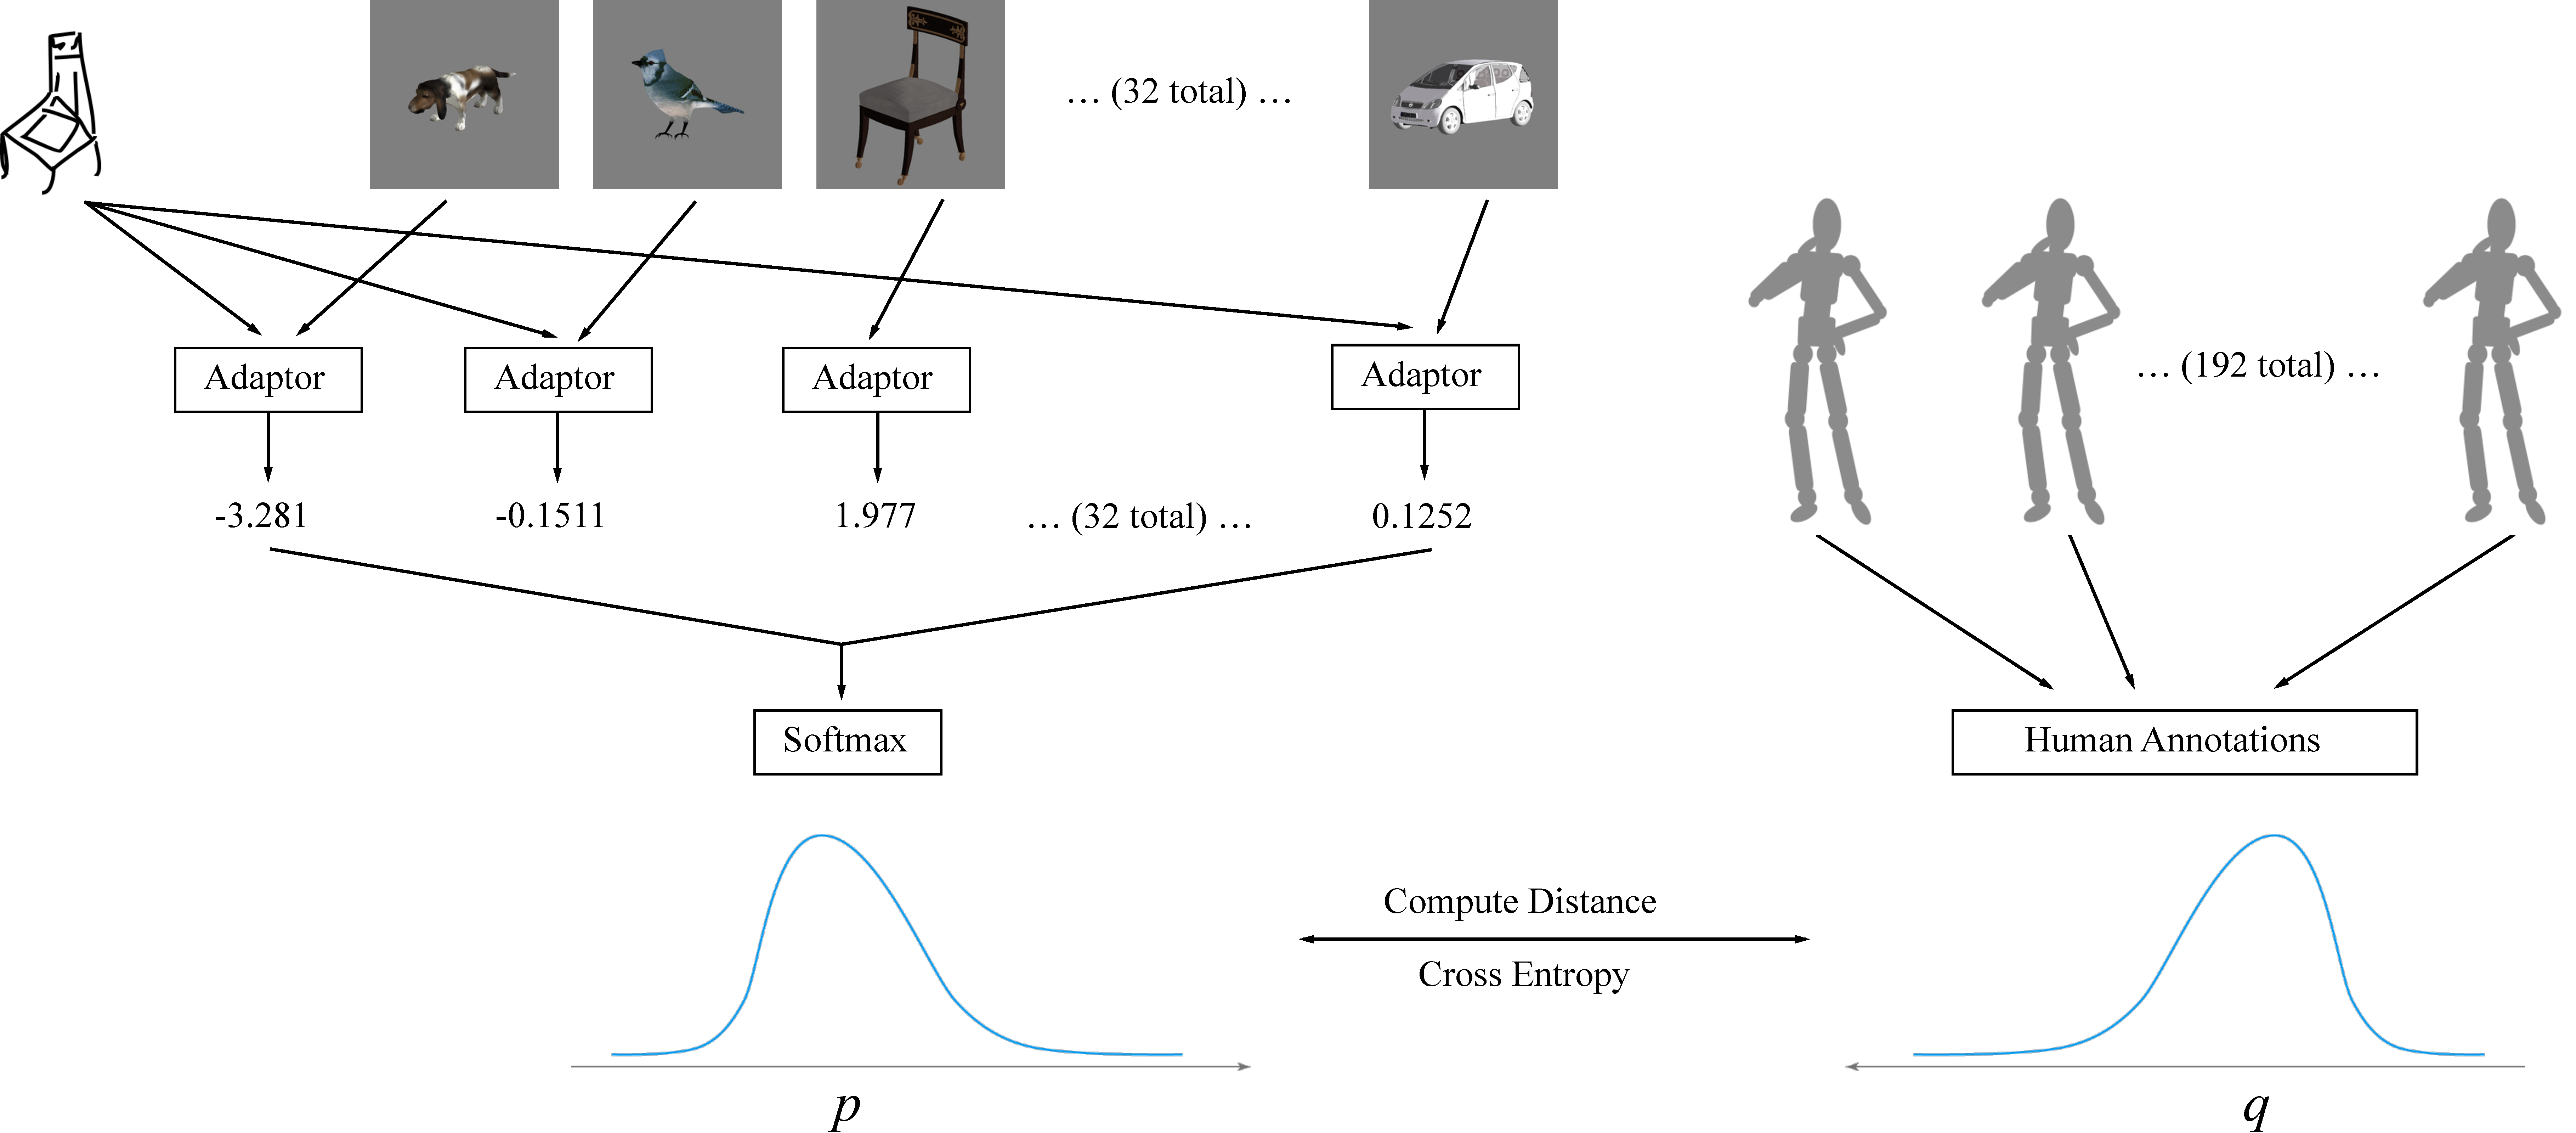
\includegraphics[width=0.95\columnwidth]{figures/adaptor_algorithm.pdf}
% \caption{The adaptor measures similarity between a given sketch and 3D object rendering. To train the adaptor, we can minimize the distance between the distribution induced from a softmax over similarities and the human annotations.}
% \label{fig:adaptor_training}
% \end{figure}

\subsubsection*{Visual encoder training}

We trained each adaptor (i.e., high, mid, low) to predict, for each sketch, a 32-dimensional vector that captures the \textit{pattern} of perceptual correspondences between that sketch and all 32 objects. 
Each encoder accepts a sketch-object pair as input and returns a real number as output (in range $(-\infty, + \infty)$), reflecting their perceptual correspondence.
We iterate over all objects in the stimulus set $\mathcal{I}$ to generate the predicted 32-vector for each sketch, and then apply softmax normalization, yielding a vector that sums to 1. 
We define the loss function, $\mathcal{L}$, to be the cross entropy loss between the predicted distribution, $q$ and the empirically estimated perceptual correspondence vector, $p$ (which also sums to 1):

\begin{equation}
    \mathcal{L} = \sum_{x \in \mathcal{I}} p(x)\log q(x)
    \label{eqn:cross_entropy}
\end{equation}

% The empirical response distribution was derived by computing the proportion of trials from the recognition experiment on which all sketches from the same context-object category (e.g., all sparrow sketches produced on close trials) was matched with each object. 
% As a consequence, this response distribution not only provides an estimate of the strength of the match between a sketch and its corresponding object, but also the pattern of confusions that human observers exhibit, thus creating a more detailed profile of recognition behavior for each adaptor to match.

This loss function explicitly encourages the adaptor to learn not only to predict the strength of the correspondence between a sketch and the object it was intended to depict (measured by correct matches during recognition), but also to predict its correspondence to all of the other objects (measured by the pattern of confusions during recognition).

We use the Adam optimization algorithm \cite[]{kingma2014adam} (learning rate = 1e-4) over minibatches of size 10 for 100 epochs, where an epoch is a full pass through the training set. 
After training each adaptor for 100 epochs, we freeze the model with the best performance on a validation set. \footnote{As a property of the input domain, the gradients with respect to adaptor parameters are very small (1.51e-4 $\pm$ 2.61e-4), inevitably resulting in poor learning (we can reproduce this effect from several intializations). We find that naively increasing the learning rate led to unstable optimization, but that multiplying the loss by a large constant $C$ leads to a much smoother learning trajectories and good test generalization. Critically, increasing the learning rate and multiplying the loss by a constant are not equivalent for second moment gradient methods. In practice, $C =$ 1e4.} 

\subsubsection*{Generating encoder-based estimates of perceptual correspondence between sketches and objects}

To generate sketch-object correspondence scores for sketches in each test split, we first pass each sketch-object pair into a visual encoder, yielding a single image-level correspondence score lying in the range $(-\infty,+\infty)$. 
To map these raw image-level scores to the appropriate range for a correspondence score ($[0,1]$), we first z-score them ($f(x) = \frac{x - \bar{x}}{\mathrm{s}}$), then apply the logistic function ($f(x)= \frac{1}{1+e^{-x}}$).
These normalized image-level correspondence scores are then averaged across all sketches belonging to the same object-context category, yielding 32 objects x 32 sketches x 2 contexts  = 2048 model-based perceptual correspondence scores for each visual encoder variant (i.e., high, mid, low).

% To compute this score for a visual encoder variant and object, each test-set sketch from a given object-context category is passed in with this object to the visual encoder module, yielding

% \mwu{We split the datasets of images and sketches into three groups: a training set, a validation set, and a test set. Post training, we use the parameters from the epoch with the highest validation accuracy i.e. early stopping ADD CITATION. During training, the model never sees any test data.}

% \subsubsection*{Pragmatic inference}

% The social inference must be able to evaluate the degree of perceptual correspondence between each object in context and any sketch it could produce, where the set of producible sketches consists of those in the test set (i.e., not used to train the visual encoder). Using this information, it outputs a distribution of scores over all test-set sketches, where the scores reflect each sketch's relative communicative utility.

% Combining the two modules, we can define the sketcher, $\mathcal{S}$ to be a decision-theoretic agent that produces sketches, $s$, by soft-maximizing a utility function, $U$, given a particular object referent, $o$:

% \begin{equation}
% \mathcal{S}(s|o) \propto \exp\{{U(s,o)\}}
% \end{equation}

% The utility function of our context-sensitive sketcher, $U_{S_1}$, trades off the extent to which a given sketch is informative to an imagined viewer, $\mathcal{V}$, with the cost of producing that sketch, $C(s)$. This notion of informativity is defined by the (natural log) probability that a viewer would select the true object given the sketch and all objects in context. In our experiments, the cost of a sketch is operationalized as the amount of time taken to produce it, though in principle other metrics could be used (e.g., the number of strokes, proportion of canvas filled).

% \begin{equation} 
% U_{S_1}(s, o) = w_i \ln \mathcal{V}(o|s) - w_c C(s)
% \end{equation}
% where $w_i$ and $w_c$ are latent parameters weighting the influences of the sketch's perceptual properties and cost, respectively.

% The viewer ($\mathcal{V}$) is assumed to decide between objects in context proportional to the perceptual correspondence between each object and the current sketch, $\textrm{sim}(s,o)$, which is scaled by a latent parameter $\alpha$.

% \begin{equation} 
% \mathcal{V}(o|s) \propto \exp\{\alpha \cdot \textrm{sim(s, o)}\}
% \end{equation}
% where $\alpha$ is a scaling parameter determining the assumed optimality of the listener's decision policy: as $\alpha \rightarrow \infty$, the listener is more likely to choose the object with highest perceptual correspondence to the sketch.

% We also consider a \textit{context-insensitive} sketcher $S_0$ agent that aims to maximize the absolute perceptual correspondence between their sketch and the target, without taking the  distractors into account. Accordingly, the utility function of this context-insensitive sketcher is defined in terms of $\textrm{sim}(s,o)$ instead of informativity to $\mathcal{V}(o|s)$.

% In our full sketcher model we combine these two agents by inferring a mixture weight parameter, $w_{prag}$, that interpolates between their two utilities:  

% \begin{equation} 
% I(s,o) = w_{prag} \cdot \ln \mathcal{V}(o | s) + (1-w_{prag}) \cdot \textrm{sim}(s,o)
% \end{equation}

% Combining the utilities in this way captures the intuition that a communicative sketcher seeks to produce a sketch that both resembles the target object and distinguishes the target from the distractors.

% After algebraically simplifying, the full utility is:

% \begin{equation}
% U(s,o) =  w_p \cdot  f(s,o) - w_c \cdot C(s)
% \end{equation}

% Each communication task trial is defined by a context containing four objects and a sketch. There are two attributes of each trial that are required for any variant of our model to be able to generate predictions given a context: (1) the perceptual correspondence between the sketch to each object in context and (2) the cost of producing the sketch.


\subsubsection*{Model comparison}

In order to test the contribution of each component of our sketcher model, we conducted a series of lesion experiments and formal model comparisons.
To quantify the evidence for one model over another, we computed Bayes Factors:
the ratio of likelihoods for each model, integrating over all their respective parameters under the prior:
$$BF = \frac{\int P(D | M_1, \theta_1)P(\theta_1)}{\int P(D | M_2, \theta_2)P(\theta_2)}$$
Unlike classical likelihood ratio tests, which use the maximum likelihood, the Bayes Factor naturally penalizes models for their complexity \cite{wagenmakers2018bayesian,jefferys1992ockham}.
We placed uninformative uniform priors over all five parameters required to specify our models: a discrete choice over alternative approaches to computing perceptual correspondance: 
$$m \sim \textrm{Unif}\{\textrm{``empirical''}, \textrm{``high''}, \textrm{``mid''}, \textrm{``low''}\}$$
and over the continuous latent parameters, 
$$w_i, w_c, w_d, \alpha \sim \textrm{Unif}(0, 50).$$ 
To compute the likelihood function $P(D | M, \theta)$ for a speaker model $M$ under parameters $\theta$, we perform exact inference for our sketcher model using (nested) enumeration and sum over all test set datapoints within a crossvalidation fold. 

% There are several possible methods to approximate Bayes Factors when exact evaluation of the integral is intractable. We compare two independent methods to check the robustness of our estimate: annealed importance sampling and exact enumeration over a discretized grid of parameters. Annealed importance sampling (AIS; \cite{neal2001annealed}) is a Monte Carlo algorithm that is commonly used to estimate the partition function, or marginalized likelihood, of probabilistic models. Because the integral is dominated by a typical set near the region of high likelihood, AIS uses an MCMC chain to construct a sequence of intermediate distributions interpolating between a tractable initial distribution (in our case, the prior) and intractable target distribution: we set the number of steps to 2000 and take the expectation over 48 independent samples from this procedure for every model of interest, using the implementation provided in the probabilistic programming language WebPPL. We can then obtain Bayes Factors to compare models by taking ratios of these estimates.

% We compare our results from AIS to a more exact but brute-force approach: 

Specifically, we compute the exact likelihood at every point on a discrete grid of parameters.
This is of particular interest for nested model comparisons, e.g. comparing our full model to a context-insensitive variant.
Rather than computing the full marginalized likelihood for both models, we can use the Savage-Dickey method \cite{wagenmakers2010bayesian} to simply compare the posterior probability against the prior at the nested point of interest (e.g. $w_c = 0$) for the full model.

To evaluate the contribution of pragmatic inference, we begin by comparing the pragmatic sketcher model using empirically estimated perceptual correspondences to nested ``cost-insensitive'' ($w_c = 0$) and ``context-insensitive'' ($w_d = 0$) variants. To evaluate the contribution of visual abstraction, we then proceed to compare the three visual encoder variants that adapt features from different layers of VGG-19, marginalizing over all other parameters. Finally, we perform the same context and cost lesion experiments on the full model, employing best-performing visual encoder (i.e., ``high'').

\subsubsection*{Evaluating model predictions}

% To further interpret the findings of our model comparison, we examined posteriors over the inferred parameters of the best-performing model and also computed posterior predictives to evaluate its behavior on several measures of interest: (1) the absolute rank of target sketch category; (2) probability assigned to sketches from the congruent context, i.e. $P(\textrm{`close' sketches} | \textrm{`close' context)} + \textrm{P(`far' sketches} | \textrm{`far' context})$; and (3) the mean cost of predicted sketches. 

We implemented our models and conducted inference in the probabilistic programming language WebPPL \cite{goodman2014design}.
We use MCMC to draw 1000 samples from the joint posterior with a lag of 0, discarding 3000 burn-in samples.
We constructed posterior predictive distributions by computing each measure of interest (i.e., target rank, context congruity, sketch cost) over the test data set, for every MCMC sample.
To estimate standard errors on predictions across models, we employed the following procedure to account for three nested sources of variation: variation across trials within a test split, variation across the parameter posterior within a test split, and variation across test splits.  
% estimation of measures on the data for a particular parameter setting and test split, variation across the parameter posterior for a test split, and variation across test splits. %% may want to include more detail about how exactly this was done. 
Specifically, for each model variant and for each test split we bootstrap resampled trials with replacement from the test dataset 1000 times to estimate the mean and standard error on each measure of interest, marginalizing over MCMC samples from the parameter posterior. 
We applied inverse-variance weighting to aggregate these estimates of the mean and standard error across test splits, such that test splits with lower variance contribute more than do splits with higher variance, yielding an overall estimate of the mean and standard error for each measure of interest, for each model variant. 
We estimated the half-widths of the 95\% confidence interval for each measure of interest under the the assumption of normality for the sampling distribution of the mean.

}

\showmatmethods % Display the Materials and Methods section

\acknow{Thanks to Dan Yamins and the Stanford CoCo Lab for helpful comments and discussion.}

\showacknow{} % Display the acknowledgments section

% \pnasbreak splits and balances the columns before the references.
% Uncomment \pnasbreak to view the references in the PNAS-style
% If you see unexpected formatting errors, try commenting out \pnasbreak
% as it can run into problems with floats and footnotes on the final page.
%\pnasbreak

% Bibliography
\bibliography{references}

\end{document}
